\documentclass{svmult}

\usepackage[utf8]{inputenc}
\usepackage[table]{xcolor}
\usepackage{url}
\usepackage{hyperref}

\usepackage[numbers]{natbib}
%\usepackage[switch]{lineno}

\usepackage{amsmath} % assumes amsmath package installed
\usepackage{amssymb}  % assumes amsmath package installed

\usepackage{enumerate}
\usepackage{paralist} %for inline lists

\usepackage{array}
\usepackage{amsmath}

\usepackage{subfigure}

\usepackage{pseudocode}
\usepackage{alltt}

%diagrams
\usepackage{tikz}
\usetikzlibrary{shapes,trees}

\usepackage{lscape}

\usepackage[draft]{fixme}
\fxusetheme{color}

%%%%%%%%%%%% Custom macros %%%%%%%%%%%%%

%Name of the speaker in a chat
\newcommand{\chatN}[1]{{\footnotesize \textsf{#1}}}
\newcommand{\concept}[1]{{\footnotesize \texttt{#1}}}

\newcommand{\stmt}[1]{{\footnotesize $\langle$\stmttt#1\relax$\rangle$}}
\newcommand{\rawstmt}[1]{{\footnotesize \stmttt#1\relax}}
\def\stmttt#1 #2 #3\relax{{\tt#1} {\bf{\tt #2}} {\tt #3}}

\newcommand{\setstmt}[1]{{\footnotesize [\setstmttt#1\relax]}}
\def\setstmttt#1,#2\relax{\rawstmt{#1}, \rawstmt{#2}}

\newcommand{\ie}{{\textit{i.e.~}}}
\newcommand{\cf}{{\textit{cf~}}}
\newcommand{\eg}{{\textit{e.g.~}}}

%------------------------------------------------------------------------- 

\begin{document}
%\linenumbers

% Alternate row background in tables
\rowcolors{2}{gray!10}{white}

\title*{Towards Grounding Human-Robot Interaction}

\author{
Séverin Lemaignan,
Rachid Alami,
Amit Kumar Pandey,
Matthieu Warnier,
Julien Guitton
}
\authorrunning{Séverin Lemaignan et al.}

\institute{ 
	Séverin Lemaignan, \and Rachid Alami \and Amit Kumar Pandey \and Matthieu Warnier \and Julien Guitton
	\at
	CNRS - LAAS, 7 avenue du Colonel Roche, F-31077 Toulouse, France\\
	Université de Toulouse, UPS, INSA, INP, ISAE, LAAS, F-31077 Toulouse, France\\
	\email{surname.name@laas.fr}
}

\maketitle

\listoffixmes

\clearpage

\setcounter{minitocdepth}{2}
\dominitoc


\begin{abstract}
TDB.
\end{abstract}



%%%%%%%%%%%%%%%%%%%%%%%%%%%%%%%%%%%%%%%%%%%%%%%%%%%%%%%%%%%%%%%%%%%%%%%%%%%%
%%%%%%%%%%%%%%%%%%%%%%%%%%%%%%%%%%%%%%%%%%%%%%%%%%%%%%%%%%%%%%%%%%%%%%%%%%%%
\section{Introduction}

\subsection{Grounding the Human Interaction: the Challenges}

{\em Aperitif time. Sitting down in its comfortable armchair, Tom gives a look
at the empty table. ``{\em Hey robot, put two glasses and this bottle on the
tray!}''. ``{\em And bring that over there.}''. The robot wonders ``{\em The
Martini or the Porto?}''. ``{\em Bring both!}'' answers Tom. The robot prepares
the order and smoothly bring the tray to the table.}

\begin{figure}%[!ht] 
	\centering
	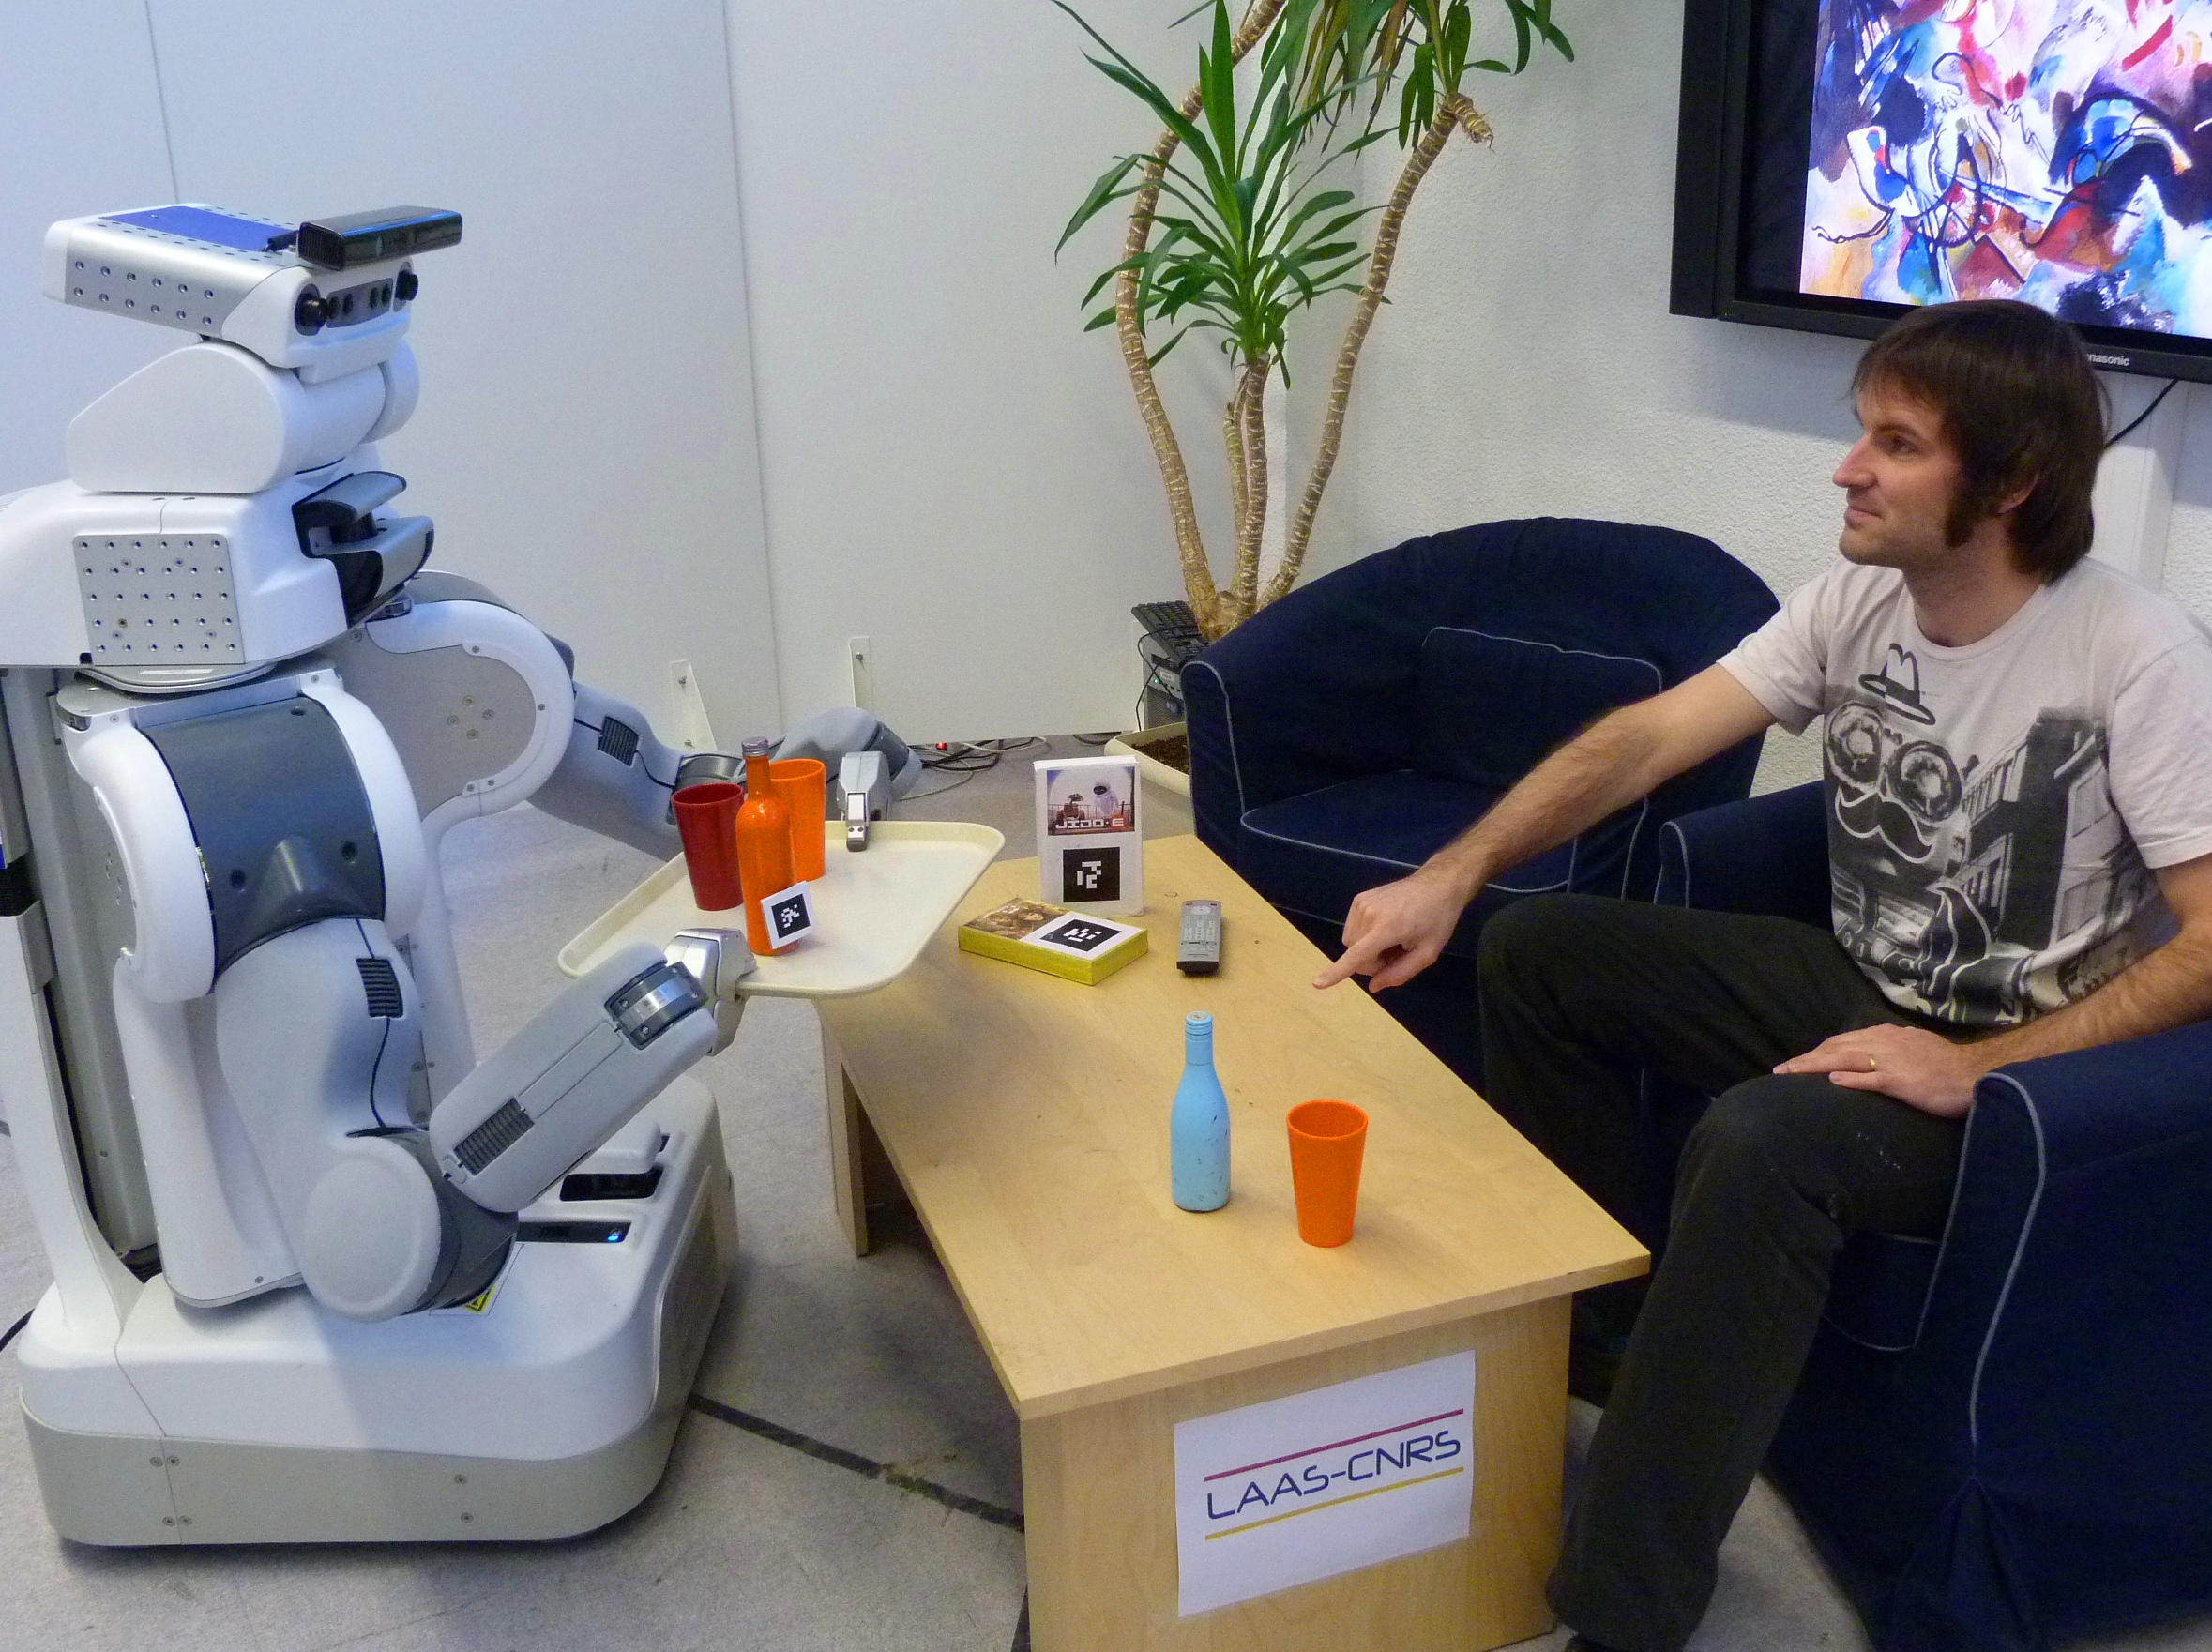
\includegraphics[width=0.8\linewidth]{figs/aperitif_time.jpg} 
	\caption{Interacting with the robot in an everyday situation: the human 
	asks for help in vague terms, the robot takes into account the human's 
	spatial perspective to refine its understanding of the question.} 
	\label{fig|vpt} 
\end{figure}

While the dream of the robot-servant could be questioned, this kind of natural
interaction (illustrated in Fig.~\ref{fig|vpt}) is a short-term target for the
human-robot interaction community.

This simple scenario belongs to the broad class of \emph{interactive
manipulation problems}: several agents have a (more or less implicit) joint goal that requires some
sort of cooperation to be successfully achieved. These problems are often iterative
(step-by-step resolution, questions-answers,...) and involve both dialogue and
manipulation.


\begin{figure}[htb]
\centering
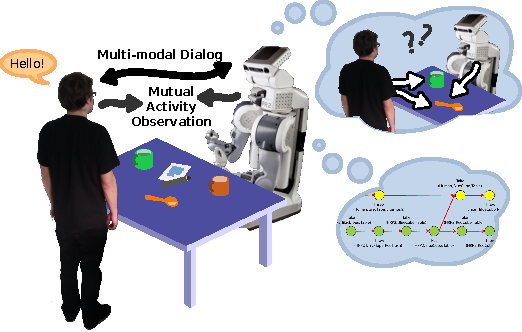
\includegraphics[width=9cm]{figs/grounding_robot.pdf}
\caption{Robot reasoning about HRI and anticipation of human activities:
  sources of information are multi-modal dialogue and observation of
  the environment and the human activities}
\label{fig|hri-dec}
\end{figure}

Figure~\ref{fig|hri-dec} illustrates some of the aspects of the interaction.
From the robot perspective, several cognitive skills are involved: dialogue
processing through different modalities, verbal and deictic (what does the
human say? what attitude -- glances, postures, gestures... -- does he
express?), acquisition and maintainance of one or several models of the
environment, not only from the robot point of view, but also from the other
agents' points of view, anticipation (what are the intentions of the human? Can
I predict and anticipate his actions?), planning and control (how would I
proceed further towards the goal?), monitoring of the other agents' activities
and the overall progress of the task (do we have an effective cooperation?)

We can look back to our initial ``\emph{Aperitif Time}'' scenario and analyse
it along these lines.

What are the prerequisites for such a sentence --``Robot, put two glasses and
this bottle on the tray''-- to be understood by the robot, correctly
interpreted in the spatial context of the interaction, and eventually
transformed into a set of actions?


\fxfatal{TO FILL}
...

We summarizes these challenges in four categories:

\begin{enumerate}

	\item how to build and maintain a consistent model of the current
	situation, acquired through perception or deduction from previous
	perceptions,

	\item how to build an unambiguous representation of concepts (objects,
	agents, actions...) underlying the interaction, and practical for
	decision-making processes,

	\item how to establish the joint goal(s), how to build and maintain
	iteratively shared (human-robot) plans, 

	\item how to refine and execute the computed plans, and how to monitor
	those achieved by its human partner?

\end{enumerate}


This chapter focuses on the points {\it 1} and {\it 2}. It presents techniques,
developed and used on several real robots, for the creation of a set of
environment models suitable for grounded situation interpretation,
decision-making and control.

The two other items are however equally important to achieve a rich and legible
interaction. Thus we shall briefly overview the global architecture of a robot
able to interact with humans\fxwarning{Shall we stay very broad or focus on
*our* implementation?} before really focusing on the grounding issues.

%%%%%%%%%%%%%%%%%%%%%%%%%%%%%%%%%%%

\subsection{An Architecture for Grounding}
 
\begin{figure*}[thpb]
  \centering
  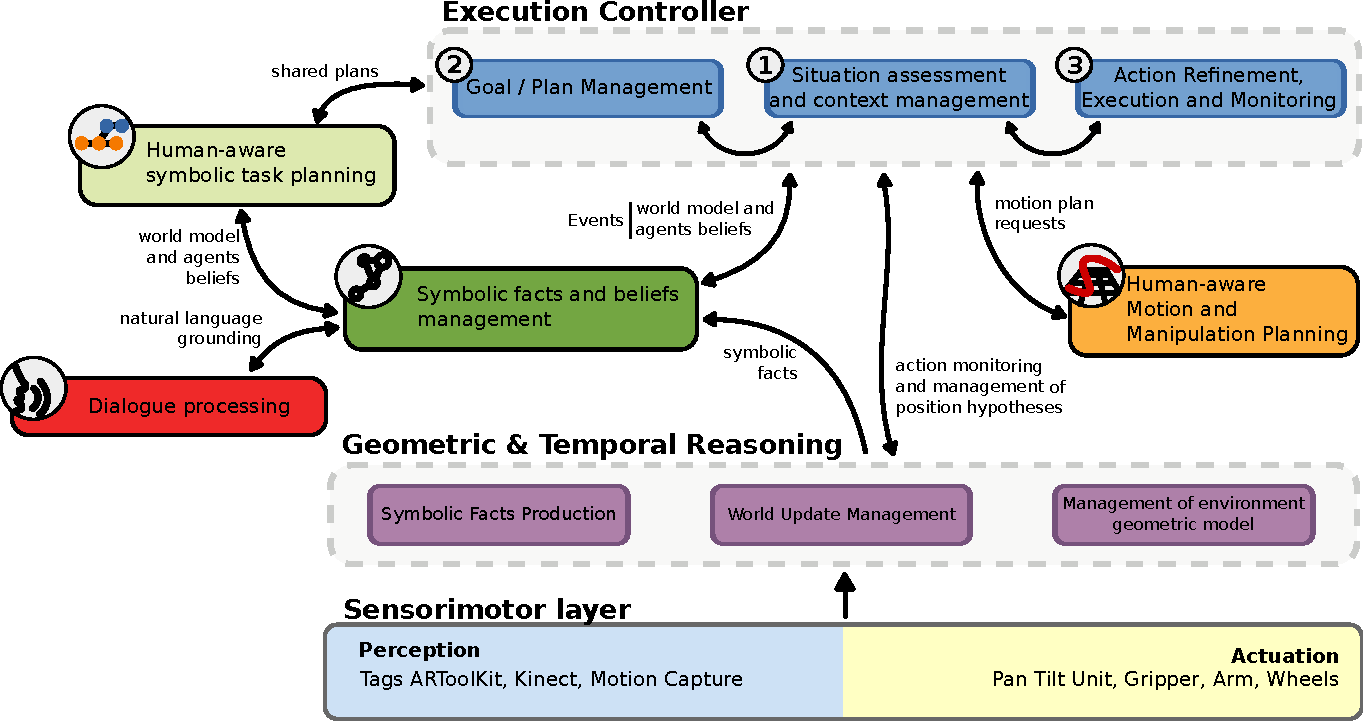
\includegraphics[width=1.0\textwidth]{./figs/architecture-overview.pdf} \\
  \caption {Architecture of the robot control system}
  \label{fig|archi}
\end{figure*}

Figure~\ref{fig|archi} gives an overview of the overall decisional layer of
our robots~\cite{Alami2011}. The sensorimotor layer (bottom) is abstracted in
an intermediate 3D geometric model where geometric (and some temporal)
reasoning take place~\cite{Sisbot2011}.

The outcomes of the geometric analysis, as well as the result of the dialogue
processing module~\cite{Lemaignan2011b}, are stored in a central knowledge
base~\cite{Lemaignan2010}. The symbolic knowledge base triggers events that are
captured by the top-level robot controller.

The controller can rely on two specialized planner: the geometric motion and
manipulation planner~\cite{Sisbot2008, Mainprice2011, Pandey2010} and the
symbolic task planner~\cite{Alili2008}.

The dialogue processing module, as well as the symbolic task planner, also
use the knowledge base to answer questions or initialize the planning domain.

During a typical interaction experiment, the robot controller decides upon a
plan to execute, requires a plan from the task planner, affects the actions to
the human and the robot, communicates the shared plan, and controls and
monitors its execution. The operation continues until the goal is achieved, is
declared unachievable or is abandoned by the human.


%%%%%%%%%%%%%%%%%%%%%%%%%%%%%%%%%%%
%% Notice on our main assumption %%
%%%%%%%%%%%%%%%%%%%%%%%%%%%%%%%%%%%

\subsubsection*{On object identification and localization}

This architecture makes one important assumption (hidden in the
\emph{Sensorimotor layer} box in Figure~\ref{fig|archi}): world entities are
assumed to be correctly \emph{perceived}, \emph{localized}, \emph{resolved} and
\emph{uniquely identified} in a \emph{repetable} way.

This means that we assume all relevant entities (\ie the objects the robot has
to interact with) to be actually perceived by the robot when they enter its
field of view (we shall come back and precisely define the \emph{field of view}
in the next section), that the entities' percepts enable a \emph{good enough}
6D localization, that these entities are properly resolved (\eg, two bottles
next to each other are perceived as two different bottles), and most
importantly that these entities are robustly identified: each time the exact
same object is seen (possibly under a different angle), it is always labelled
with the same, unique, identifier (the identifier by itself may be completely
random, and can be known at runtime only).

Concretly this assumption typically translates during experiments by tagging
each objects with a barcode-like label (some can be seen on Fig.~\ref{fig|vpt})
that allows the robot to localize and identify these objects.

Numerous works \fxfatal{Cite some of them} (some of them presented earlier in
this book) focus on dealing with the resolution and identification issues.  We
will not further discuss them here.

%%%%%%%%%%%%%%%%%%%%%%%%%%%%%%%%%%%


\subsection{Chapter overview}

This chapter walks through the on-line building and use of symbolic models of
the environment and interacting agents. As far as possible, we will try to
present the exact list of symbolic statements issued by the whole system at
runtime.

We start by introducing an approach to create symbolic models of the
environment, seen by the robot or by the other interacting agents. To the end,
we introduce \emph{Perspective Taking}~\cite{Flavell1992,Tversky1999} and some
elements of \emph{Theory of Mind}~\cite{Scassellati2002}\fxwarning{Check this
reference is relevant here} Techniques to efficiently compute perspective-aware
models of the world are presented. 

\emph{Search} and \emph{exploration} policies are also presented, along with
symbolic ways to deal with under-defined locations.

The next section focuses on the modeling of agents and agents capabilities,
including a geometric approch for the analysis of the potential of actions (we
call it the \emph{Mightabilities}) of each agent.

Section~\ref{cognitivekernel} presents a centralized knowledge base that
stores, reasons about, and asynchronously (event-driven) exposes the symbolic
facts to decision-making processes. We also discuss here the role of {\it a
priori} knowledge (the so-called \emph{common-sense knowledge}).

The following two sections~\ref{hatp} and~\ref{dialogs} present actual
applications of this approach. First, we show how the robot may
use the symbolic models for shared task planning: using each agent's model of
the world, one stream of actions per agent is generated, with synchronization
points between them. Then, we present how multi-modal (verbal and deitic)
dialogue processing is made much easier by relying on consistent symbolic
models, using semantics close to human natural language.

Bibliographical notes have been added at the end of each relevant section.  We
also present before the conclusion of the chapter other architectures dedicated
to the grounding of human-robot interaction, along with some references
regarding the specifics of the human-robot interactions.


%%%%%%%%%%%%%%%%%%%%%%%%%%%%%%%%%%%%%%%%%%%%%%%%%%%%%%%%%%%%%%%%%%%%%%%%%%%%
%%%%%%%%%%%%%%%%%%%%%%%%%%%%%%%%%%%%%%%%%%%%%%%%%%%%%%%%%%%%%%%%%%%%%%%%%%%%

\section{Building a Symbolic Model of the Environment}
\label{sec:situ}

Anchoring perceptions in a symbolic model requires perception abilities
and their symbolic interpretation. In this section we present
SPARK (\emph{SPAtial Reasoning \& Knowledge}~\cite{Sisbot2011}), a situation assessment reasoner
that generates relevant symbolic information from the geometry of the
environment with respect to relations between objects, robots and humans.

\begin{figure}[ht!]
   \begin{center}
%
       \subfigure{
           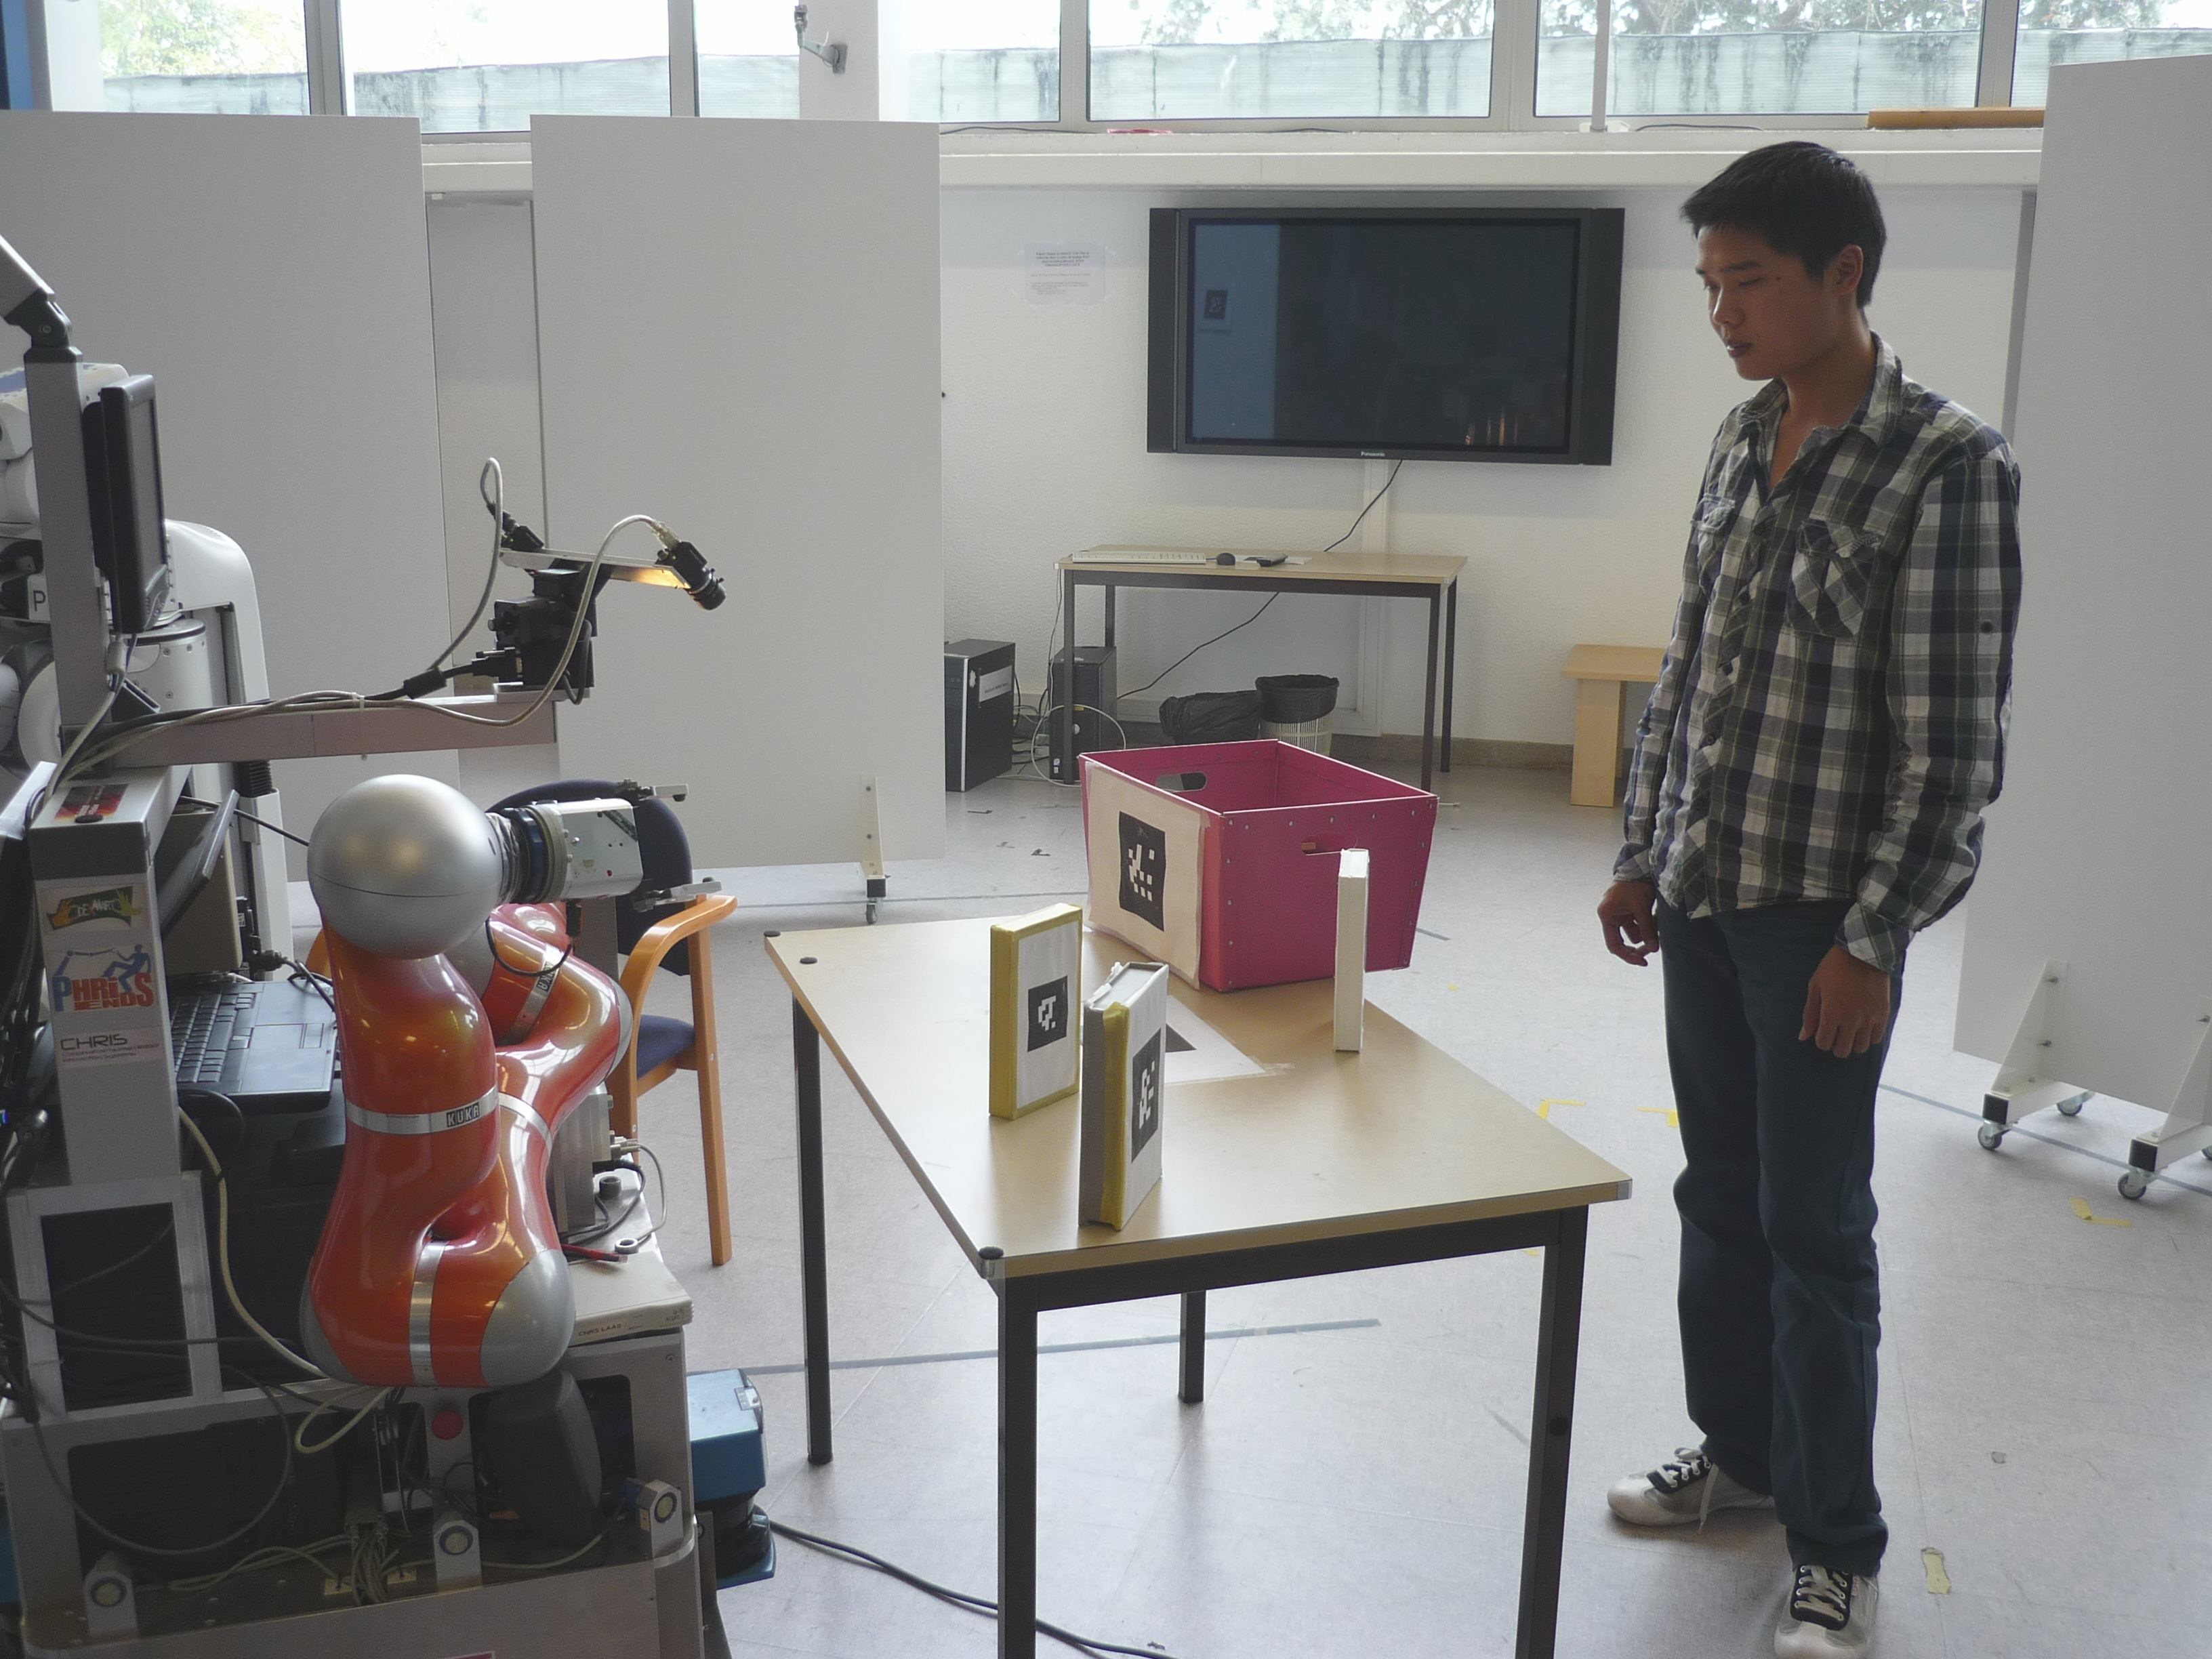
\includegraphics[width=0.5\textwidth]{./figs/etat2-P1010769_brightened-v2.jpg}
       }%
       \subfigure{%
          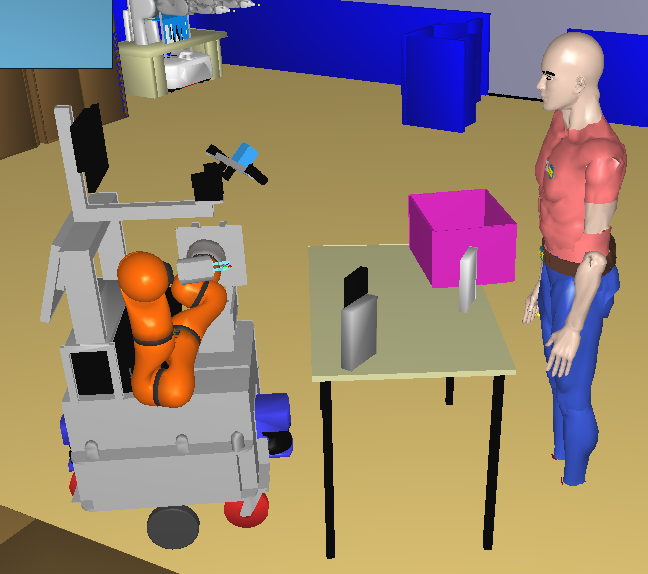
\includegraphics[width=0.43\textwidth]{./figs/etat2_photo.png}
       }\\ %  ------- End of the first row ----------------------%
%
   \end{center}

   \caption{The robot represents at runtime its environment in a 3D model resulting of the sensors' inputs fusion.}%
   \label{fig|spark}

\end{figure}

\subsection{Locations}

One way of referring to object's positions is based on human's symbolic 
descriptors, instead of using their precise position. In fact, in many cases, 
this information is the most precise information available since humans do not 
store the numeric coordinates of objects. These type of descriptors have been 
studied in the context of language grounding 
(\cite{O'Keefe1999,Matuszek2010,Regier2001,Kelleher2009,Blisard2005}). In this 
work we focus on the following relations which are computed with respect to the 
position of the agents and the objects:

\begin{itemize} 

\item \emph{Location according to an agent}: The predicate
\concept{isLocatedAt} represents spatial locations between agents and objects.
For example we say ``it is on my right, on your left, ...'' We compute these
spatial locations by dividing the space around the referent (an agent) into $n$
regions based on arbitrary angle values relative to the referent orientation.
For example, for $n = 4$ we would have the space divided into \emph{front,
left, right} and \emph{back}. Additionally, two proximity values, \emph{near}
and \emph{far}, may also be considered. The number of regions and proximity
values can be chosen depending on the context where the interaction takes
place.

\item \emph{Location according to an object}: We can also refer to object
locations with respect to other objects in the environment, such as \emph{above,
next to, in}, etc. In this work we compute three main relations based on the
bounding box and center of mass of the objects 
(Figure~\ref{fig|sprelations}): 

\begin{itemize}
	\item \concept{isOn}: computes if an object $O_1$ is on another object $O_2$ by
	evaluating the center of mass of $O_1$ according to the bounding box of $O_2$.

	\item \concept{isIn}: evaluates if an object $O_1$ is inside another object
	$O_2$ based on their bounding boxes $BB_{O_1}$ and $BB_{O_2}$.

	\item \concept{isNextTo}: indicates whether an object $O_1$ is next to another
	object $O_2$. We cannot use a simple distance threshold to determine if two
	objects are next to each other since the relation is highly dependent on the
	dimensions of the objects. For instance, the maximum distance between large
	objects (\eg two houses) to consider them as being next to each other is much
	larger than the maximum distance we would consider for two small objects (\eg
	two bottles). Thus, the relation between the dimensions and the distances of
	the objects are taken into account.  

\begin{figure} 
	\centering
	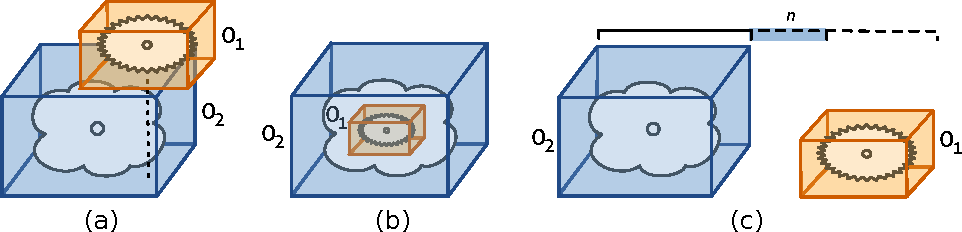
\includegraphics[width=0.95\columnwidth]{figs/spatial_relation.pdf}
	\caption{Spatial relations between two objects: (a) \concept{isOn} relation, 
	(b) \concept{isIn} relation, and (c) \concept{isNextTo} relation.} 
	\label{fig|sprelations} 
\end{figure}

\end{itemize} 
\end{itemize}

To ensure the different agent models are up-to-date, all these properties are
always computed on-line, each time the current state of the world changes.

Table~\ref{facts|sprelations} lists all the symbolic relationships that are
currently computed by the system.

\begin{table}[h]
    \centering
    \begin{tabular}{p{1.5cm}p{5cm}p{2cm}p{4cm}}
	\rowcolor{white}
    \textbf{Subject} & \textbf{Predicate} & \textbf{Object} & \emph{Notes} \\ 
    \hline
	 \concept{Location} & \concept{isAt} $\equiv$ \concept{cyc:objectFoundInLocation}  &  \concept{Location} & \\ 
	 &  $\rightarrow$ \concept{isOn} $\equiv$ \concept{cyc:above\_Touching}  &  & \\ 
	 &  $\rightarrow$ \concept{isIn}  &  & \\ 
	 &  $\rightarrow$ \concept{isNextTo}  & &  \\ 
	 \concept{Location}  & \concept{isAbove} $\equiv$ \concept{cyc:above-Generally}  &  \concept{Location}  &  inverse of \concept{isBelow} \par \concept{isOn} $\Rightarrow$ \concept{isAbove}\\ 
	 \concept{Location}  & \concept{isBelow}  & \concept{Location}  &  inverse of \concept{isAbove}
	\end{tabular}

	\caption{List of statements describing spatial relationships between
	objects. ``$\rightarrow$'' indicates sub-properties. When existing, the
	equivalent predicate in the {\sc OpenCyc} standard (prefix \concept{cyc:})
	has been added.}

\label{facts|sprelations}
\end{table}

SPARK also compute symbolic facts related to agent independent world dynamics.
The predicate \concept{isMoving} states, for each tracked entity, whether it is
currently moving or not.


\subsection{Relative placements}

While in previous section we listed several \emph{absolute} location predicate,
many topological relations are directly dependent from the observation point.

To build an agent-dependent model of the world, \emph{Perspective
Taking}~\cite{Flavell1992,Tversky1999} is employed by the reasoner to provide
the robot with the ability to put itself at the human's place (by moving a
camera in the geometric model) and to reason about the world from different
perspectives.


Through perspective taking, SPARK computes for each agent a symbolic
description of the relative positioning of objects in the environment (table
\ref{facts|relative}).

\begin{table}[h]
	\centering
	    \begin{tabular}{p{1.5cm}p{6cm}p{1.5cm}l}
		\rowcolor{white}
		\textbf{Subject} & \textbf{Predicate} & \textbf{Object} & \emph{Notes} \\
		\hline
	 \concept{Location}  & \concept{hasRelativePosition}  & \concept{Location} & \\ 
	 & 	$\rightarrow$ \concept{behind} $\equiv$ \concept{cyc:behind-Generally}  &  & inverse of \concept{inFrontOf}  \\ 
	 &  $\rightarrow$ \concept{inFrontOf} $\equiv$ \concept{cyc:inFrontOf-Generally}  & 	 & 	 inverse of \concept{behind}  \\ 
	 &  $\rightarrow$ \concept{leftOf}  &  &  inverse of \concept{rightOf} \\ 
	 &  $\rightarrow$ \concept{rightOf}  & 	 & 	 inverse of \concept{leftOf}  \\ 
	 \concept{Object}  & \concept{cyc:farFrom}  &  \concept{Agent} & \\ 
	 \concept{Object}  & \concept{cyc:near}  &  \concept{Agent} & 
	\end{tabular}
	\caption{List of statements describing relative spatial relationships between objects and agents.}
	\label{table|relative}
\end{table}


\subsection{Exploration policies}

To effectively maintain the model of the world, the robot may adopt context-dependent strategies to observe its environment.

We implement two categories of policies:

\begin {itemize}
\item Exploration policies: the robot exhaustively scans the surrounding environment to
  see all what can be observed.

\item Search policies: the robot looks for an specific object until it is
  detected if possible, scanning surrounding furnitures and looking in human
  hand.

\end {itemize}

The robot must also monitor events that are not directly linked to robot action
to drive world update. The robot controller uses SPARK to monitor human hand
motion and primitive action recognition (\cf section~\ref{sec|primitives}) to
detect actions like \emph{pick} and \emph{throw}.  These trigger specific
exploration behaviours.

\subsection{Uncertain Locations and Management of Hypotheses on States and Positions}

Unknown or under-defined locations are represented by the mean of randomly
generated location IDs. For instance, if the location of \concept{BottleA} has
no name, it can be stored as \stmt{bottleA isAt loc12578}, with
\concept{loc12578} a random ID. 

If the position is actually completely unknown, \concept{loc12578} has no
further informations attached to it (and can be omitted altogether). On the
contrary, if some is known about the location, it can be refined by qualifying
the location, \eg \stmt{loc12578 isAbove MyNiceTable, loc12578
owl:differentFrom MyNiceTable}. 


It is sometimes difficult or even impossible to see and/or track an object in
certain states. This happens, for instance, when the object has been put in a
container, when it is in the robot gripper or in the human hand, and more
generally in any state in which it is hidden by something else. Our robot has a
model of the possible symbolic states for an object (whether the object is on a
furniture, in an agent hand, in a container, etc.).  According to the robot
perception of what has happened since the object was last seen, the robot tries
to maintain a belief of the current possible symbolic states and their
associated probabilities for this object. Such information can be used to
update the beliefs using input from exploration, dialog, human visual focus,
etc.

SPARK currently provides a simple implementation of such a functionality. The
only managed hypotheses are \emph{in container} and \emph{in agent hand}. We
can have only one hypothesis at the same time. Hypothesis validity is checked
geometrically in case of incoming perception values.



The robot reasons on possible positions for non perceived objects. These
hypotheses are refined using new input from dialogue, human action and focus of
attention. Currently, we manage at most one hypothesis per object. This
hypothesis is produced by robot controller through an inference on robot or
human action. In case of perception conflicts with low probability for the
current hypothesis, the robot controller will break this hypothesis and delete
corresponding symbolic fact in the knowledge base.

\subsection{Related work}

Building and updating an intermediate 3D geometric model is common in robotic
architecture. However, framework like SPARK, used as a hub for both sensor
fusion and geometric reasoning, are less common.

SPARK can be compared to the \emph{Grounded Situation Model} (GSM) introduced
by Mavridis and Roy~\cite{Mavridis2005} in the sense that they both provide an
amodal physical representation of the world used as a mediator between the
sensor space and symbolic models. They have however different features: while
GSM enables representation of time and imaginary objects (whose existence is
hinted by verbal assertions from a human, also called \emph{presupposition
accomodation}), SPARK offers a richer 3D model that enables the computation of
several spatial relationships between objects and an effective implementation
of perspective taking capabilities.

On the other hand, applications of spatial reasoning~\cite{O'Keefe1999} are
multiple. Ithas been used for instance for natural language processing for
applications such as direction recognition ~\cite{Kollar2010,Matuszek2010} or
language grounding~\cite{Tellex2010}.~\cite{Skubic2004} presented a spatial
reasoner integrated in a robot which computes symbolic positions of objects.


%%%%%%%%%%%%%%%%%%%%%%%%%%%%%%%%%%%%%%%%%%%%%%%%%%%%%%%%%%%%%%%%%%%%%%%%%%%%
%%%%%%%%%%%%%%%%%%%%%%%%%%%%%%%%%%%%%%%%%%%%%%%%%%%%%%%%%%%%%%%%%%%%%%%%%%%%

\section{Building a Model of Agents}
\label{grounding_agents}

Building a grounded symbolic model of the physical environment does not suffice
in general to fully ground the human-robot interaction.

We divide the process of building models for agents into two categories:
operations related to the assessment of the current situation (for instance,
\emph{What does the human do? What does he see?}), and operations related to
the estimation of potential actions (for instance, \emph{Which regions could
the human reach if I want to hand over an object?}). We call these
potentialities of action \emph{Mightabilities}.

\subsection{Agent Capabilities}

There are a number of common properties for a robot and a human related to
their capabilities in a given situation: they can both reach, grasp, look at,
point at, etc. In our context, we group robots and humans into a single category.
Thus, we define agents as entities that can act in the environment and
manipulate it. In this work we focus on the following capabilities from each
agent's perspective:

\begin{itemize}

\item \emph{Sees}: An important ability to know about an agent is to predict
``what it can see'', \ie what is within its field of view (FOV). A robot being
able to compute this information can then act accordingly. An example would be
a clarification scenario where the human is searching for an object and the
robot is able to infer that he/she is looking for the one that is not visible
(otherwise the user would not be searching for it).  In
Figure~\ref{fig::sparkRepresentations}\emph{a} the field of view of a person is
illustrated with a grey cone (broader one). While he is able to see the two
small boxes on the table in front of him, the big box on his right is out of
his FOV, and therefore, he is not able to see it. 

\item \emph{Looks At}: this relation corresponds to what the agent is focused
on, \ie where its focus of attention is directed. This model is based on a
narrower field of view, the field of attention (FOA). 
Figure~\ref{fig::sparkRepresentations}\emph{a}
shows the field of attention of a person with a green cone (narrower one). In
this example only the grey box satisfies the \concept{looksAt} relation.

\item \emph{Points At}: verifies whether an object is pointed at by an agent.
This relation is particularly useful during interaction when one of the agents
is referring to an object saying ``this" or ``that" while pointing at it.
 
If a larger object occludes a smaller one while an agent is pointing at them, the
outcome of the evaluation will result only in one relation, \ie \stmt{agent\_01
pointsAt object\_01} since the small one is not visible to the agent.  On the
contrary, if the small object is in front of the big one, then both objects
will satisfy the relation, which may generate an ambiguity (which object the
agent refers to?) that should be solved through higher level reasoning (\eg
context analysis or clarification through verbal interaction).

\item \emph{Reachable}: it allows the robot to estimate the agent's capability
to reach an object, which is fundamental for task planning. For example, if the
user asks the robot to give him/her an object, the robot must compute a transfer
point where the user is able to get the object afterward. 
Figure~\ref{fig::sparkRepresentations}\emph{b} shows different reachability postures for each object
on the table. In the example, the bottle and the box are both reachable for the
human, but the teddy bear is too far. Instead, from the robot's perspective,
the teddy bear is reachable for it, while the bottle is not.

\end{itemize}

\begin{figure*}[!t]
	\begin{center}
	\subfigure[]{
		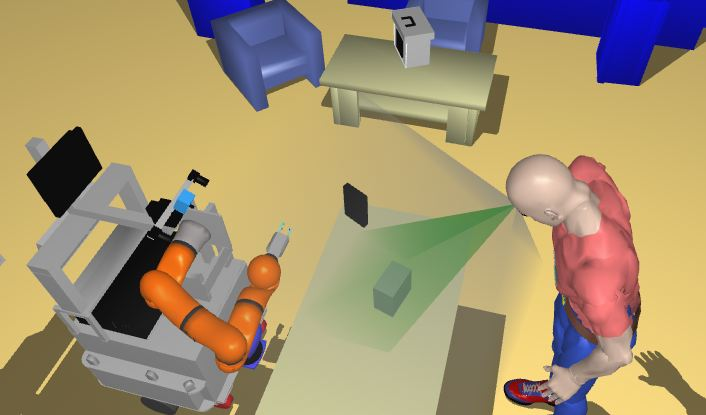
\includegraphics[width=0.4\linewidth]{figs/looks.jpg} 
		\label{(a)}
	}
	\subfigure[]{
		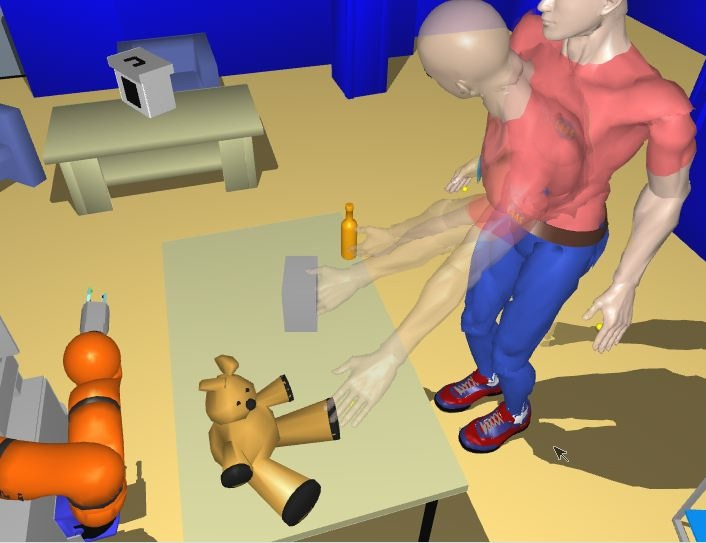
\includegraphics[width=0.35\linewidth]{figs/reach.jpg}
		\label{(b)}
	} 
	\caption{(a) Field of view (FOV) and the field of attention (FOA) of the human. (b) Different reaching postures for the human.}
	\label{fig::sparkRepresentations}
	\end{center}
\end{figure*} 


While the first three relations (\concept{sees}, \concept{looksAt} and
\concept{pointsAt}) are computed through a model based approach, the latter one
is based on the Generalized Inverse Kinematics with pseudo inverse
method~\cite{Nakamura90,Baerlocher04} to find a collision free posture for the
agent where its end-effector is at the center of the object within a given
tolerance.

Tables~\ref{facts|capabilites} and~\ref{facts|reachabilities} summarize the
predicates produced by SPARK during the agent capabilities analysis phase.

\begin{table}[h]
	\centering
		\begin{tabular}{p{2cm}p{4.5cm}p{2cm}p{3.5cm}}
		\rowcolor{white}
		\textbf{Subject} & \textbf{Predicate} & \textbf{Object} & \emph{Notes} \\
		\hline
		 \concept{Agent}  & \concept{looksAt}  & \concept{SpatialThing} \\
		 \concept{Agent}  & \concept{sees}  &  \concept{SpatialThing}  &    \\ 
		 \concept{SpatialThing}  & \concept{isInFieldOfView}  &  \concept{xsd:boolean}  & via inference: \par \stmt{myself sees *} $\Leftrightarrow$ \stmt{* isInFieldOfView true} \\ 
		 \concept{Agent}  & \concept{pointsAt} $\equiv$ \concept{cyc:pointingToward}  & \concept{SpatialThing} \\ 
		 \concept{Agent}  & \concept{focusesOn}  &  \concept{SpatialThing}  &  via inference: \par \concept{looksAt} $\wedge$ \concept{pointsAt} $\Rightarrow$ \concept{focusesOn}

	\end{tabular}
	\caption{List of facts describing the attentional state of an agent. \concept{looksAt} is interpreted as an object \emph{being in the field of attention} of an agent. An object is \concept{see}n if it is visible for the agent without moving the head (ie, in \emph{field of view}).}
	\label{facts|capabilites}
\end{table}

\begin{table}[h]
	\centering
		\begin{tabular}{p{2cm}p{4.5cm}p{2cm}p{3.5cm}}
		\rowcolor{white}
		\textbf{Subject} & \textbf{Predicate} & \textbf{Object} & \emph{Notes} \\
		\hline
		\concept{SpatialThing}  & \concept{isVisibleByMovingHead}  &  \concept{xsd:boolean}  \\ 
		\concept{Agent} & \concept{seesWithHeadMovement} &  \concept{Object} & via inference: \par \stmt{myself seesWithHeadMovement *} $\Leftrightarrow$ \stmt{* isVisibleByMovingHead true} \\
		\concept{Agent} & \concept{cannotSeeWithHeadMovement} & \concept{Object} &  via inference: \par \stmt{myself cannotSeeWithHeadMovement *} $\Leftrightarrow$ \stmt{* isVisibleByMovingHead false} \\ 
		\concept{Object}  & \concept{isReachable} & \concept{xsd:boolean}  \\ 
		\concept{Agent} & \concept{reaches} &  \concept{Object} & via inference: \par \stmt{myself reaches *} $\Leftrightarrow$ \stmt{* isReachable true} \\ 
		\concept{Agent} & \concept{cannotReach} & \concept{Object} & via inference: \par \stmt{myself cannotReach *} $\Leftrightarrow$ \stmt{* isReachable false}

	\end{tabular}
	\caption{List of statements describing action potentialities for an agent.}
	\label{facts|reachabilities}
\end{table}


Table~\ref{facts|agentstate} lists the remaining symbolic facts that are produced and maintained by SPARK related to the general state of the agent.

\begin{table}[h]
	\centering
	\begin{tabular}{p{2cm}p{5cm}p{2cm}}
		\textbf{Subject} & \textbf{Predicate} & \textbf{Object} \\
		\hline
		\concept{Agent} & \concept{hasIn\{Left|Right\}Hand}  &  \concept{GraspableObject} \\ 
		\concept{Agent} & \concept{hasPosture}  &  \concept{Posture} \\
		\concept{Agent} & \concept{currentlyBodilyDoes}  &  \concept{Action}
	\end{tabular}
	\caption{List of statements describing the state of an agent in general. The \concept{currentlyBodilyDoes} predicate states the current action of the agent, be it intentional or not.}
\end{table}


% \begin{table}[h]
% 	\centering
% 	\begin{tabular}{p{2cm}p{5cm}p{2cm}}
% 		\textbf{Subject} & \textbf{Predicate} & \textbf{Object} \\
% 		\hline
% 		\concept{Agent} & \concept{currentlyPerforms})  &  a action \par (\concept{Action})
% 	\end{tabular}
% 	\caption{List of facts describing the current state of a robot.}
% \end{table}

\subsection{Primitive action recognition}
\label{sec|primitives}

Monitoring human activity is crucial to maintain a coherent state of the world.
Full human action and activity monitoring is a difficult task that requires
knowledge and reasoning both on high level facts like goals, intentions and
plans, as well as bottom-up data from agent and object motions. Simple temporal
and geometric reasoning on human hand trajectories and potential objects
placements can provide some useful clues for high level human monitoring
processes. We call this temporal and geometric reasoning \emph{primitive action
recognition}.

For example, a \emph{pick}, a \emph{throw} or a \emph{place} action can be
recognized by observing that an object on table and an empty human hand are
close to each other, or that the human hand holding an object is close to a
container, etc. Human hand position is either directly perceived or inferred
from its initial perceived trajectory.  We have a simple implementation of such
a primitive action recognition in SPARK that relies on monitoring human hand
and its motion near objects or above containers.


%%%%%%%%%%%%%%%%%%%%%%%%%%%%%%%%%%%%%%%%%%%%%%%%%%%%%%%%%%%%%%%%%%%%%%%%%%%%

\subsection{Mightabilities: pro-active analysis of potentialities}

\fxfatal{Write an introduction that glues this section with the previous ones}

In human movement and behavioral psychology literatures, different types of
reach actions of the human have been identified and analyzed,
\cite{Gardner2001, Choi2004}.  Figure~\ref{fig|reaches_taxonomy} shows taxonomy
of such reaches involving simple arm-shoulder extension (arm-and-shoulder
reach), leaning forward (arm-and-torso reach) and standing reach.

\begin{figure}
  \centering
  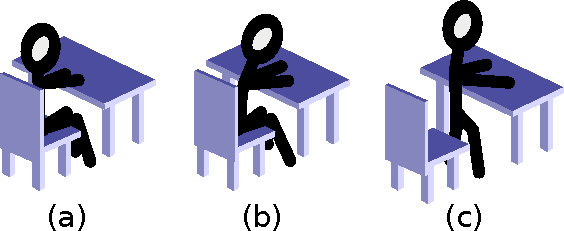
\includegraphics[width=0.5\textwidth]{./figs/reach_postures.pdf} \\
  \caption {Taxonomy of reach actions:(a) arm-shoulder reach, (b) arm-torso 
  reach, (c) standing reach.}
  \label{fig|reaches_taxonomy}
\end{figure}

Taking inspiration from such studies, we have presented the concept of
\emph{Mightability}, which stands for ``Might be Able to...'', as a framework for
\emph{multi-state visuo-spatial} perspective taking. The idea is to analyze the
various abilities of an agent such as ability to see or ability to reach, not
only from the current state of the agent, but also from a set of states, which
the agent might achieve from his current state. For this the robot applies\fxwarning{Sentence unclear}, $A_v$,
an ordered list of virtual actions, to make the agent to virtually reach a state
and then estimates the abilities $A_b \in \{See, Reach, Grasp\}$, by respecting the
environmental and postural constraints of the agent. Currently,

\[ 
A_v \subseteq \{A_v^{head}, A_v^{arm}, A_v^{torso}, A_v^{posture}, A_v^{displace}\}
\]

where

\begin{align*}
A_v^{head} & \subseteq \{PanHead, TiltHead\} \\
A_v^{arm} & \subseteq \{StretchOutArm\} \\
A_v^{torso} & \subseteq \{TurnTorso, LeanTorso\} \\
A_v^{posture} & \subseteq \{MakeStanding, MakeSitting\} \\
A_v^{displace} & \subseteq \{MoveTo\} \\
\end{align*}

When such mightability analyses are performed at the levels of cells of the
discretized 3D workspace, we term it as \emph{Mightability Maps} (MM) and when done
for the object in the space we call it \emph{Object Oriented Mightabilities} (OOM).

The robot performs mightability analyses by taking into account collision
as well as the joint limits. The information about the robot and human
positions, orientations and the 3D state of the environment is continuously
updated in our 3D representation and planning platform, Move3D \cite{Simeon2001}, which
also facilitates our robots to check intra-body and inter-body collisions
for itself and for the human model. The robot uses kinematic structures of
the agents and performs various virtual actions until the joint limits
of the neck and/or torso are reached or the collision of the torso of
the agent with the environment is detected.

\begin{figure}[ht!]
   \begin{center}
%
       \subfigure[]{%
           \label{a}
           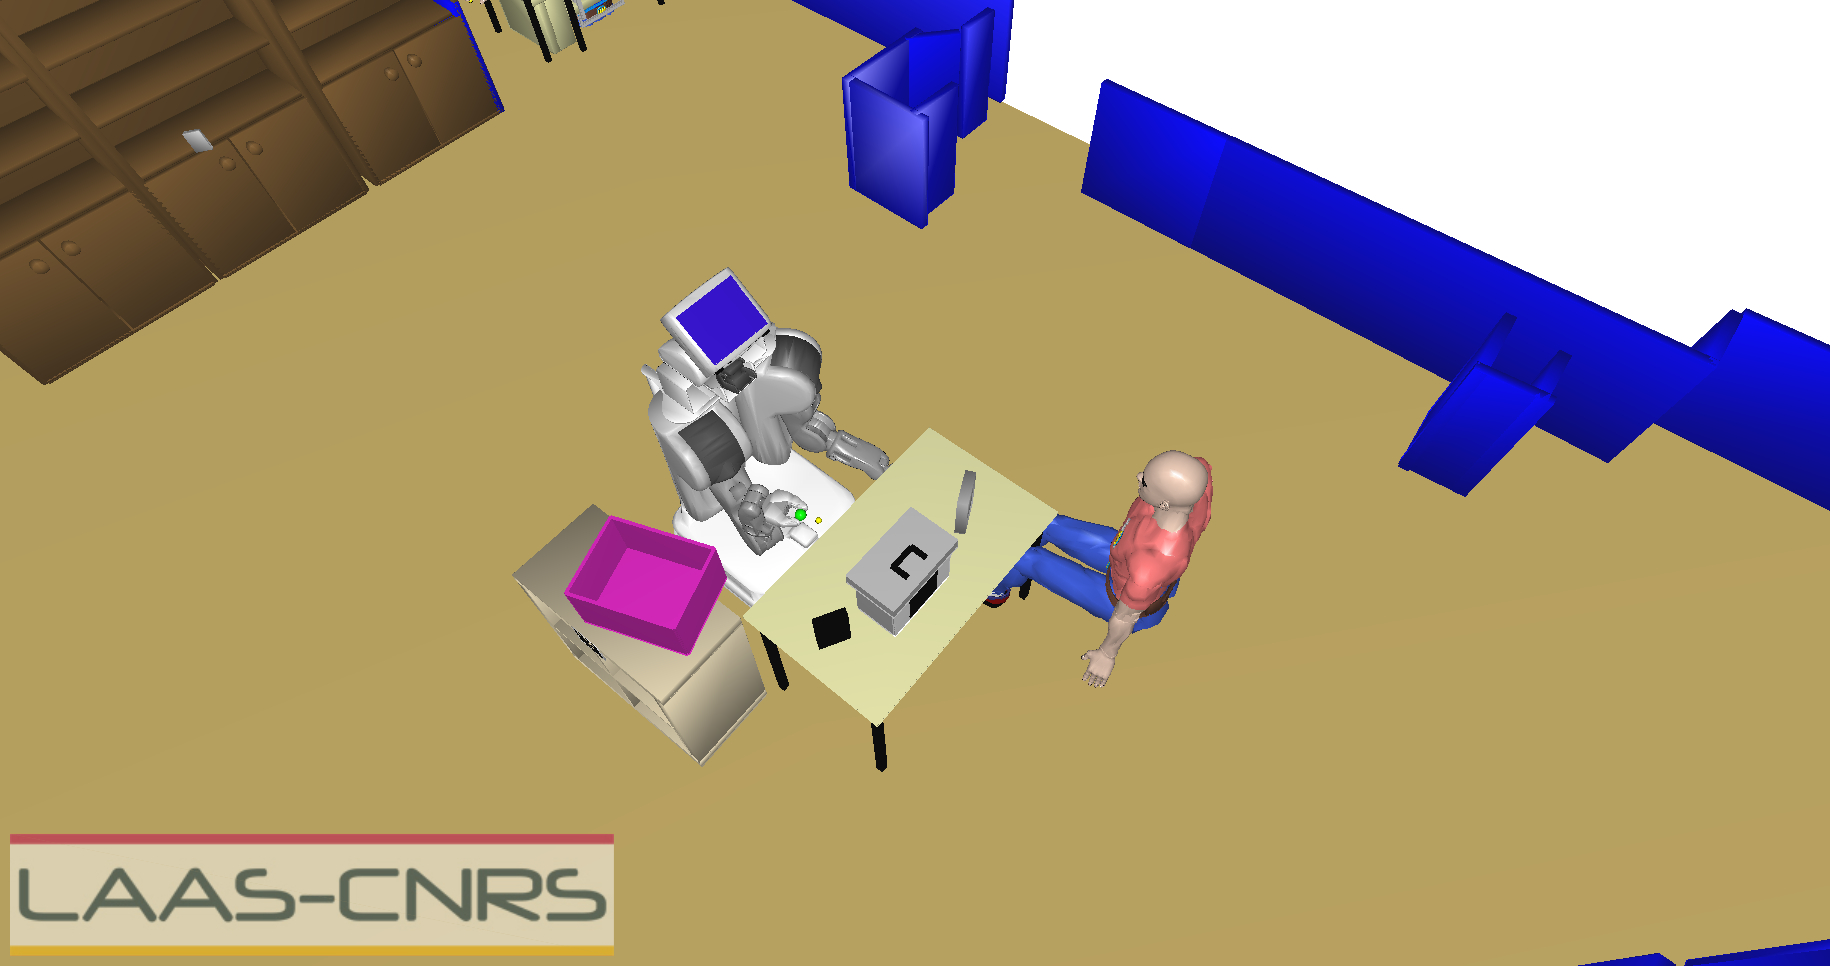
\includegraphics[width=0.5\textwidth]{./figs/mightabilities/2a.jpg}
       }%
       \subfigure[]{%
          \label{b}
          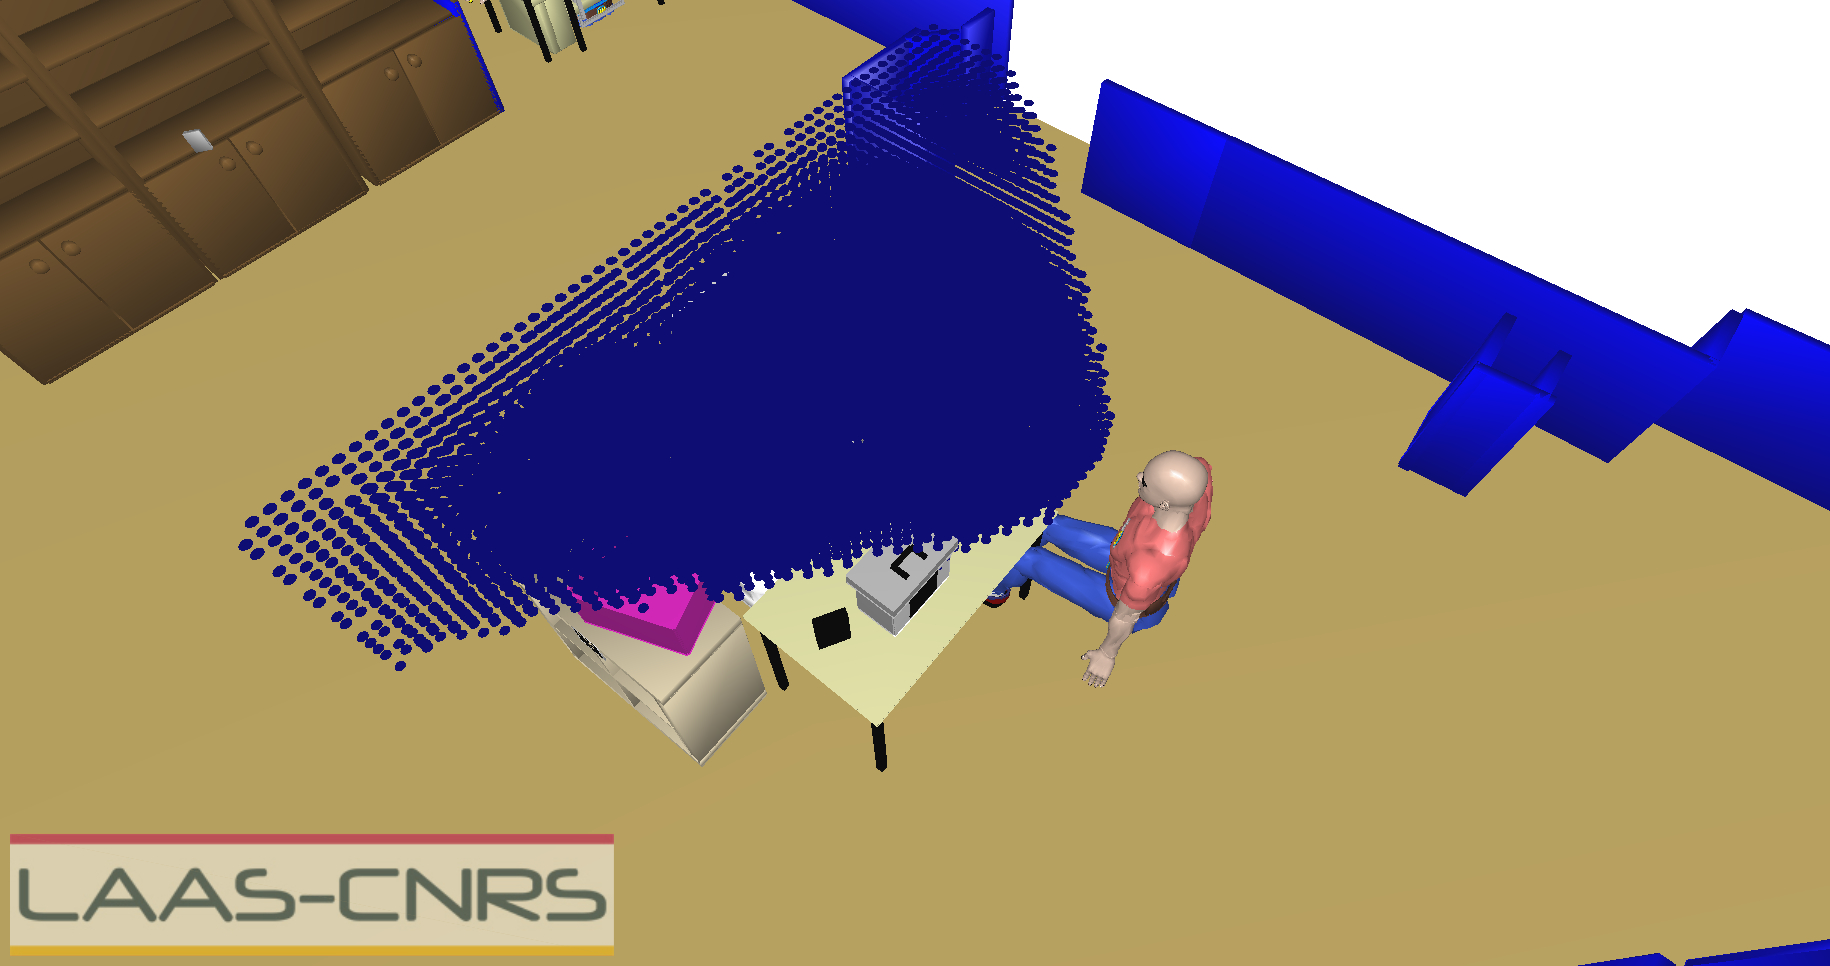
\includegraphics[width=0.5\textwidth]{./figs/mightabilities/2b.jpg}
       }\\ %  ------- End of the first row ----------------------%
       \subfigure[]{%
           \label{c}
           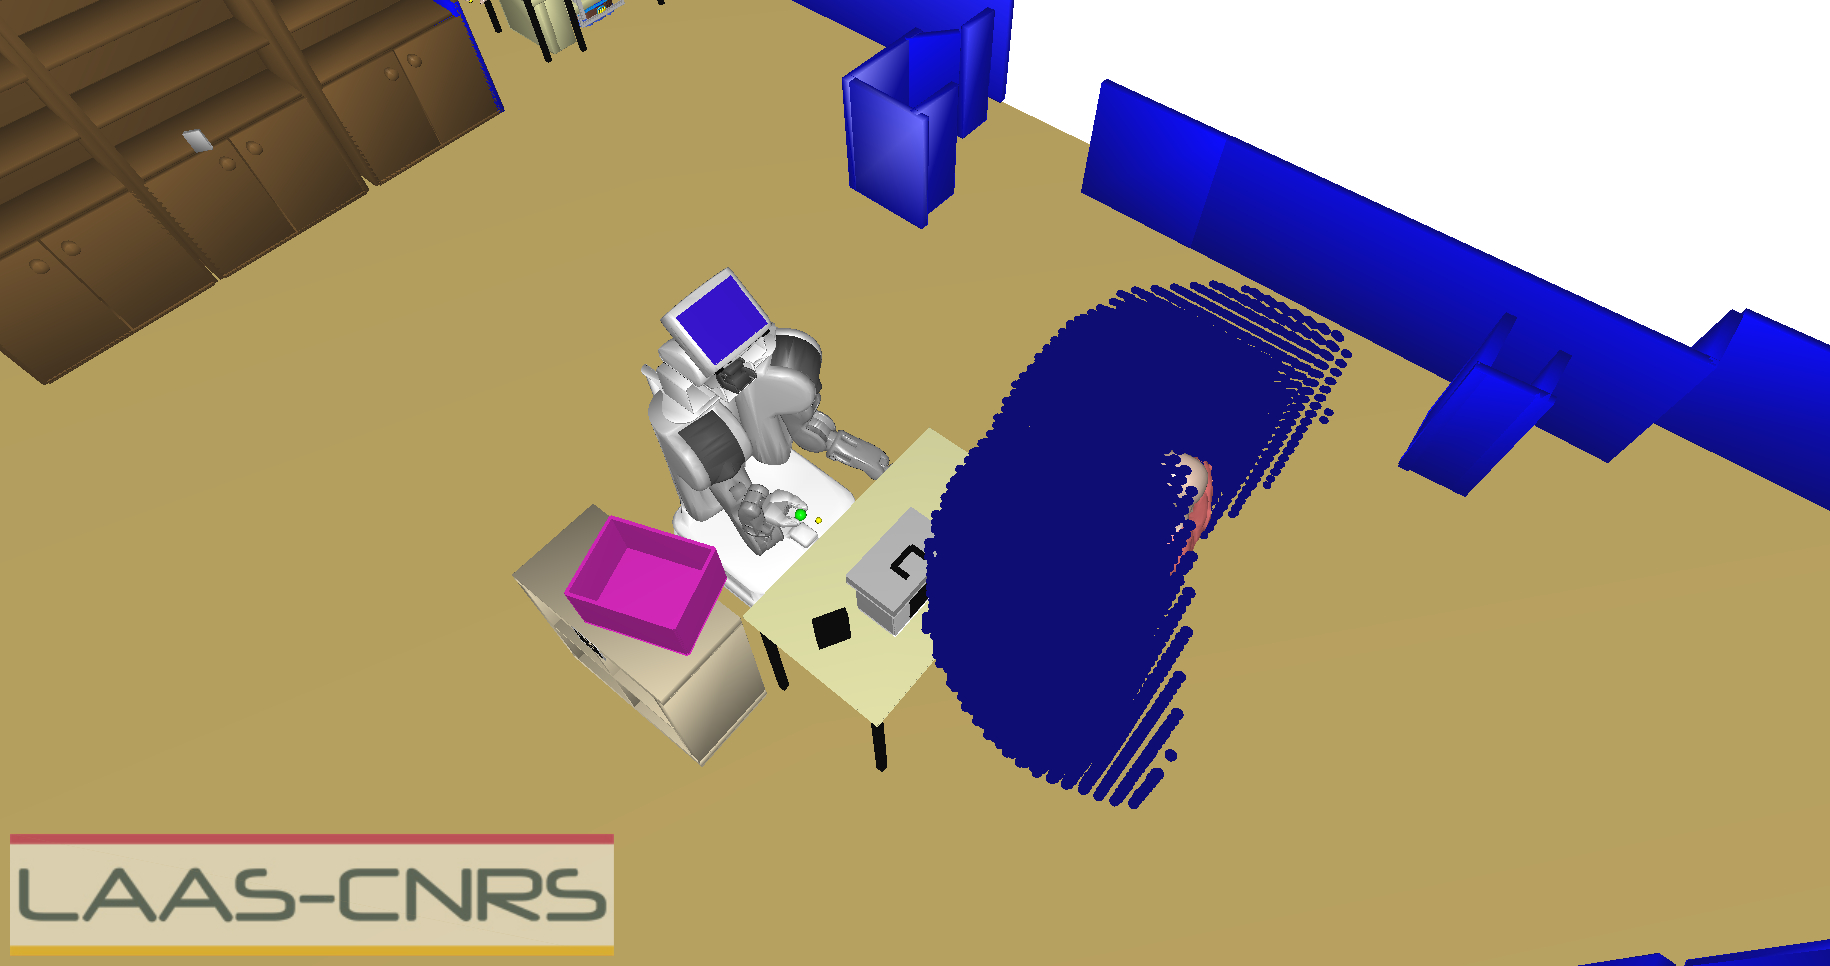
\includegraphics[width=0.5\textwidth]{./figs/mightabilities/2c.jpg}
       }%
       \subfigure[]{%
          \label{d}
          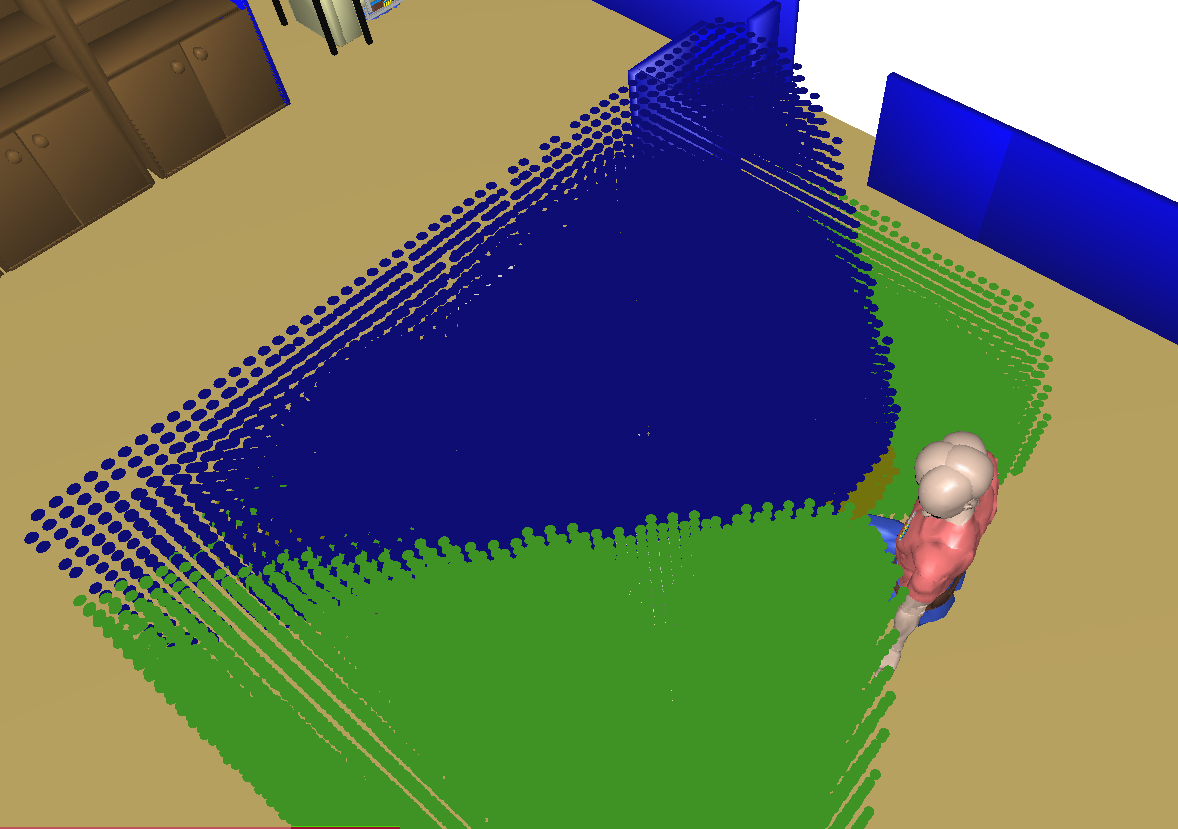
\includegraphics[width=0.5\textwidth]{./figs/mightabilities/2d.jpg}
       }\\
       \subfigure[]{%
          \label{e}
          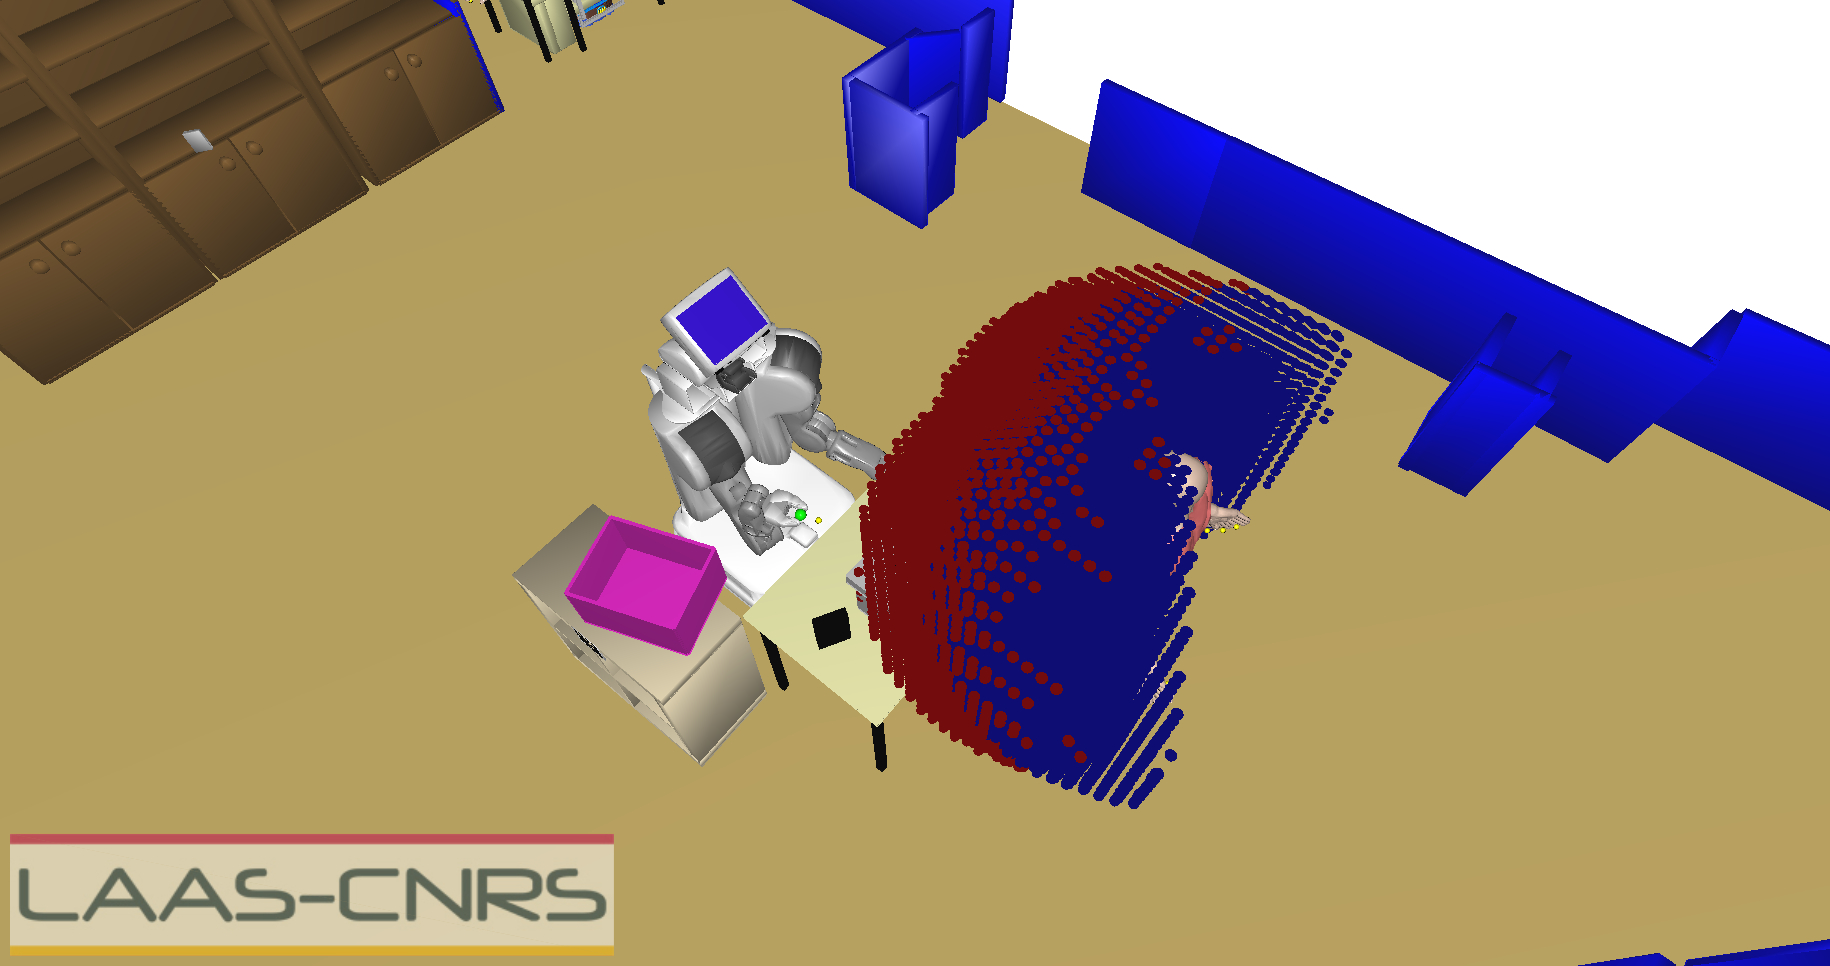
\includegraphics[width=0.5\textwidth]{./figs/mightabilities/2e.jpg}
       }   
	\end{center}

   \caption{%
		(a) 3D representation of the current world state. Mightability Maps for
		human (b) to see and (c) to reach the places in 3D from his current
		position and configuration. Because of robot's capability to perform
		multi-state perspective taking, the robot is able to estimates that if
		human will turn his head around, he can see more places (d) and if he
		will lean forward he can reach more places (e).
   }
		
   \label{fig|mightabilities}
\end{figure}

Figure~\ref{fig|mightabilities}(a) shows the current scenario.
Figures~\ref{fig|mightabilities}(b) and (c) show the MM for the places visible
and reachable by the human from his current position and configuration.

Thanks to multi-state perspective taking, the robot is also able to estimate
that if the human will just turn his head around, he will be able to see more
places (figure~\ref{fig|mightabilities}(d)) and if the human will lean forward,
he will be able to reach more space (figure~\ref{fig|mightabilities}(e)). For
reachability, the robot further distinguishes among reachable by left hand,
reachable by right hand and reachable by both hands of an agent in a particular
state.  

Mightability analysis could be performed and updated online; hence facilitate
its use for various planning and decision making components as explained below.
Mightability Map based finding candidate places for basic HRI
tasks\fxwarning{Sentence not clear}: As the robot is able to perform such
analysis for all the agents in the environment, it can use the MM to find the
candidate places to perform a set of basic HRI tasks: give, make accessible,
show, hide an object, etc. 

\begin{figure}
  \centering
  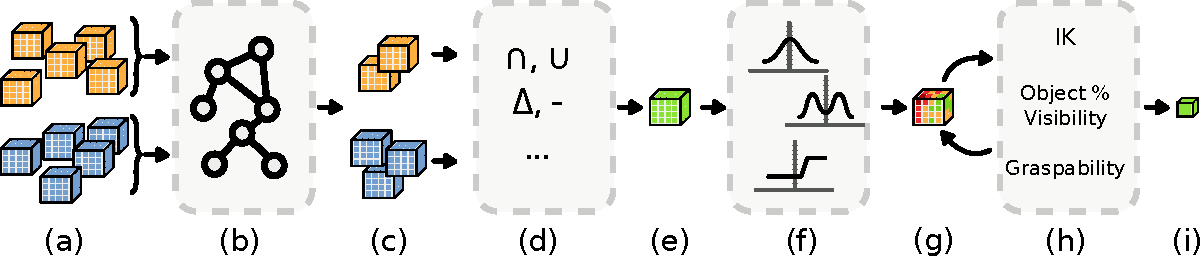
\includegraphics[width=\textwidth]{./figs/mightab-steps.pdf}

\caption { Mightability Analysis-based framework for finding a solution: (a)
Initial Mightability Maps, (b) Decision making on relevant Mightability Maps
depending on task and required comfort level of agents, (c) relevant
Mightability Maps, (d) task specific set operations, (e) raw candidate solution
set, (f) weight assignment based on spatial preferences, (g) set of weighted
candidate points, (h) applying rigorous and expensive tests on reduced search
space, (i) the feasible solution of highest weight.}

  \label{fig|mightabilities-framework}
\end{figure}


As shown in Figure~\ref{fig|mightabilities-framework}, for
finding a feasible solution of a task, robot reasons on various MM of
the involved agents and performs relevant set operations depending upon
the task.  

\begin{figure}[ht!]
   \begin{center}
       \subfigure[]{%
           \label{a}
           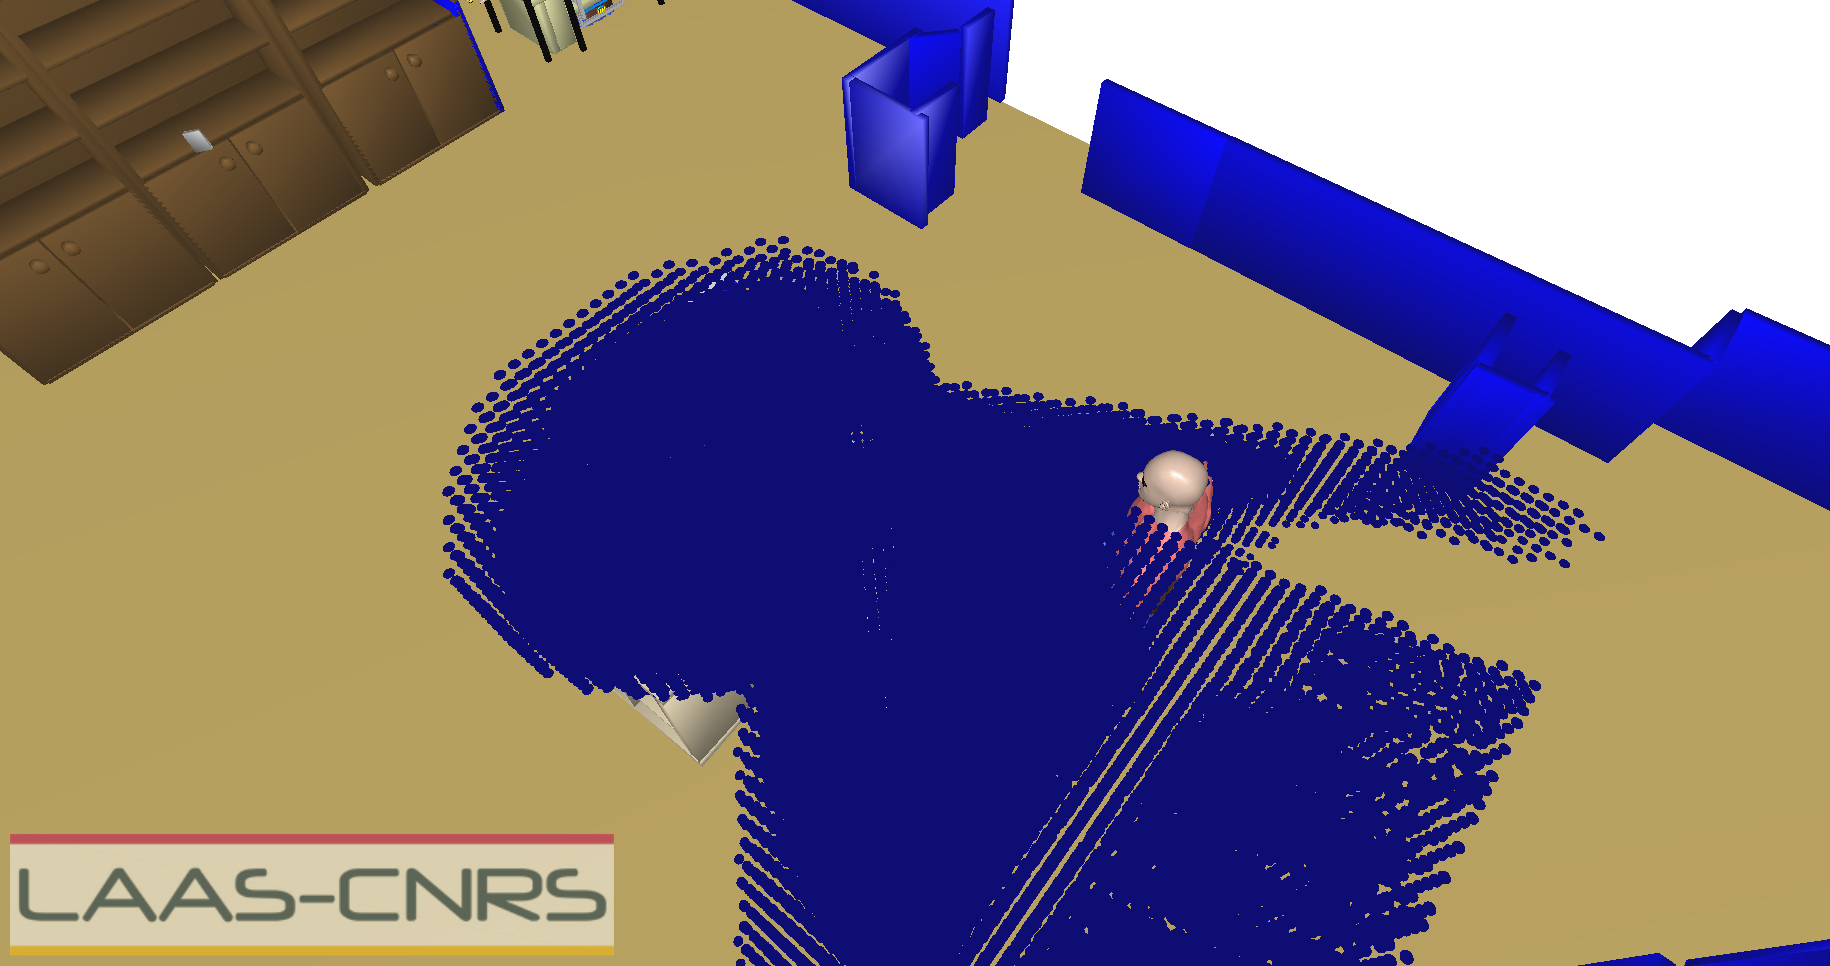
\includegraphics[width=0.5\textwidth]{./figs/mightabilities/4a.jpg}
       }%
       \subfigure[]{%
          \label{b}
          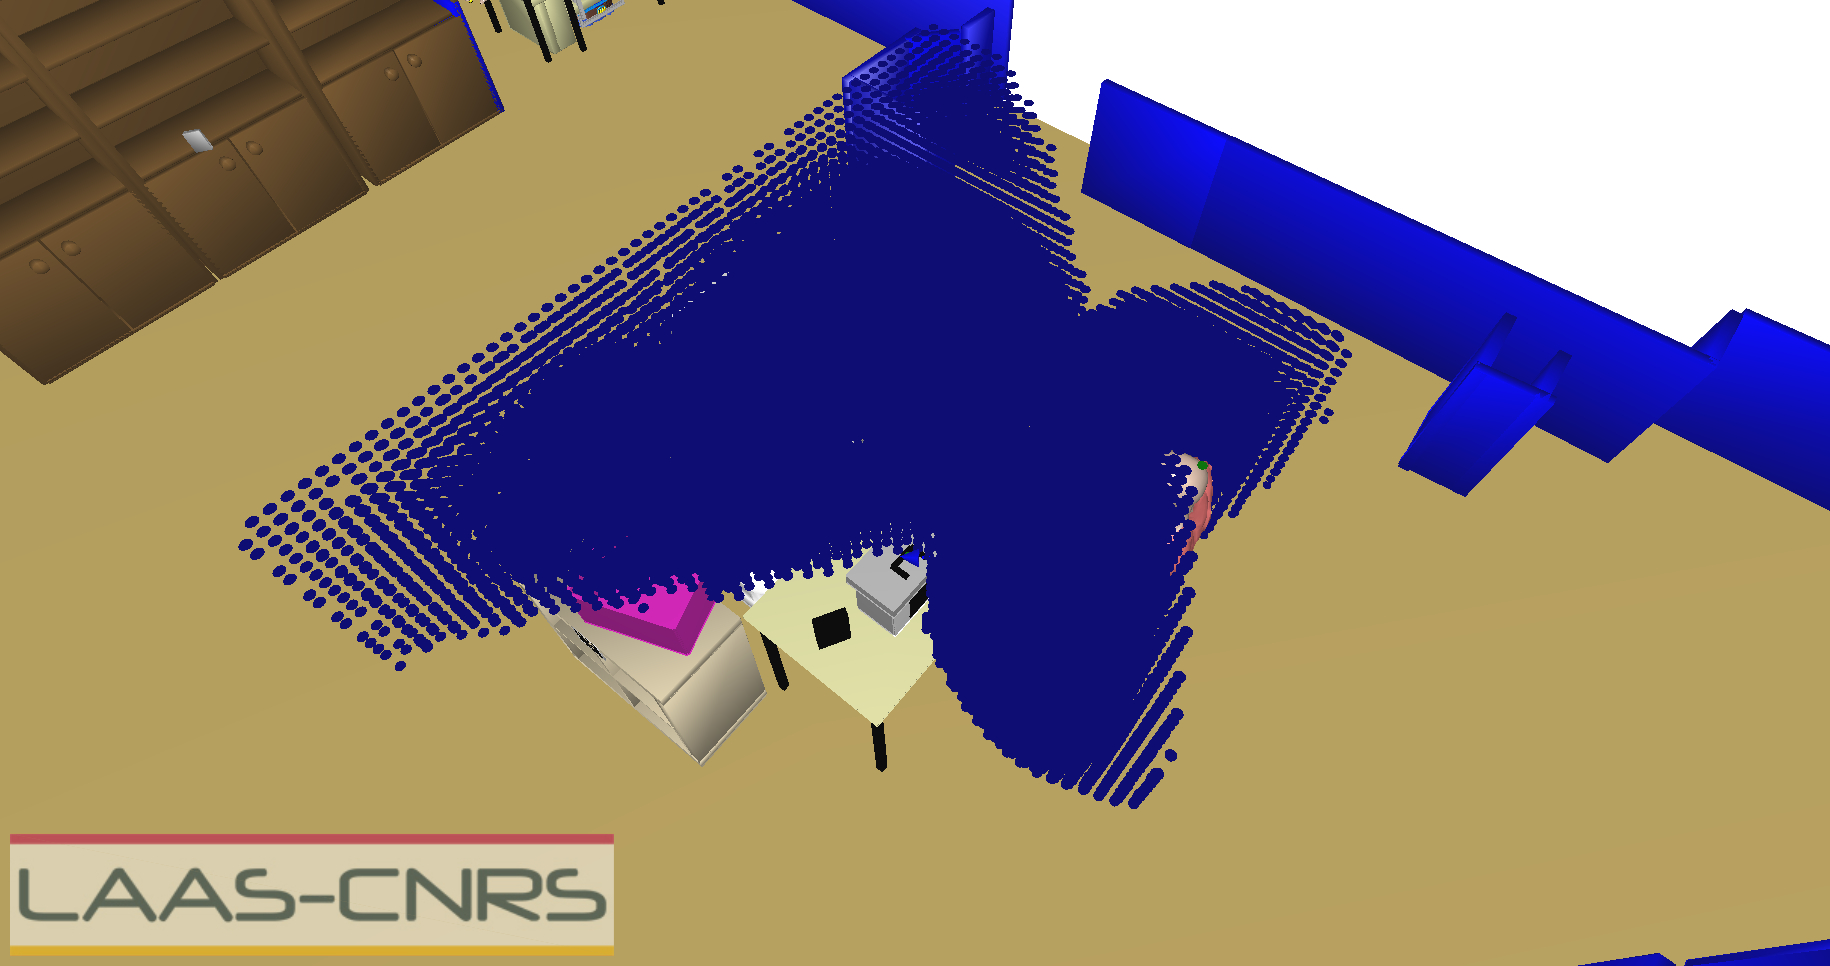
\includegraphics[width=0.5\textwidth]{./figs/mightabilities/4b.jpg}
       }\\ %  ------- End of the first row ----------------------%
       \subfigure[]{%
           \label{c}
           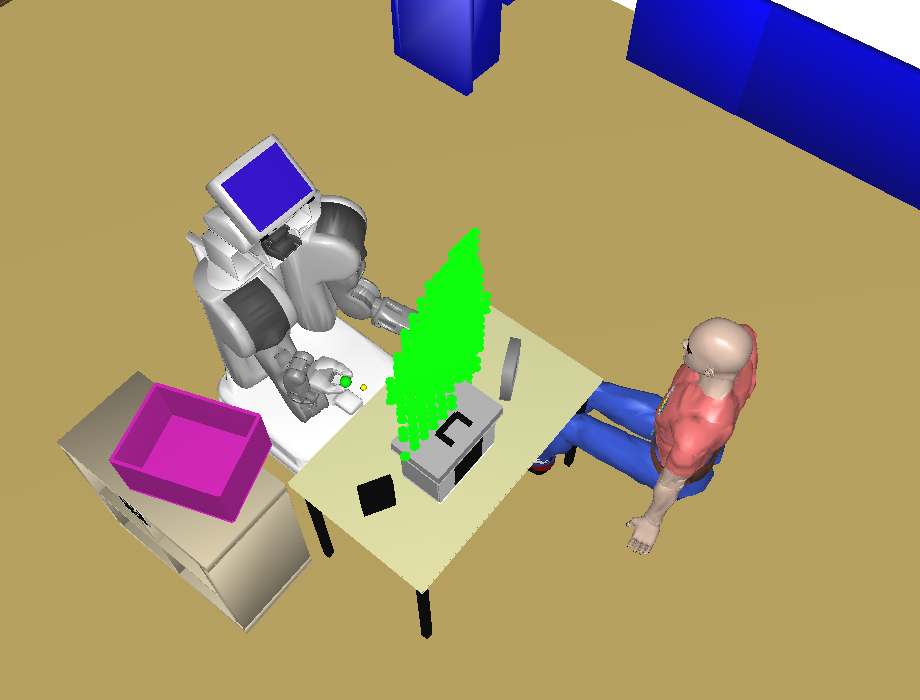
\includegraphics[width=0.5\textwidth]{./figs/mightabilities/4c.jpg}
       }%
       \subfigure[]{%
          \label{d}
          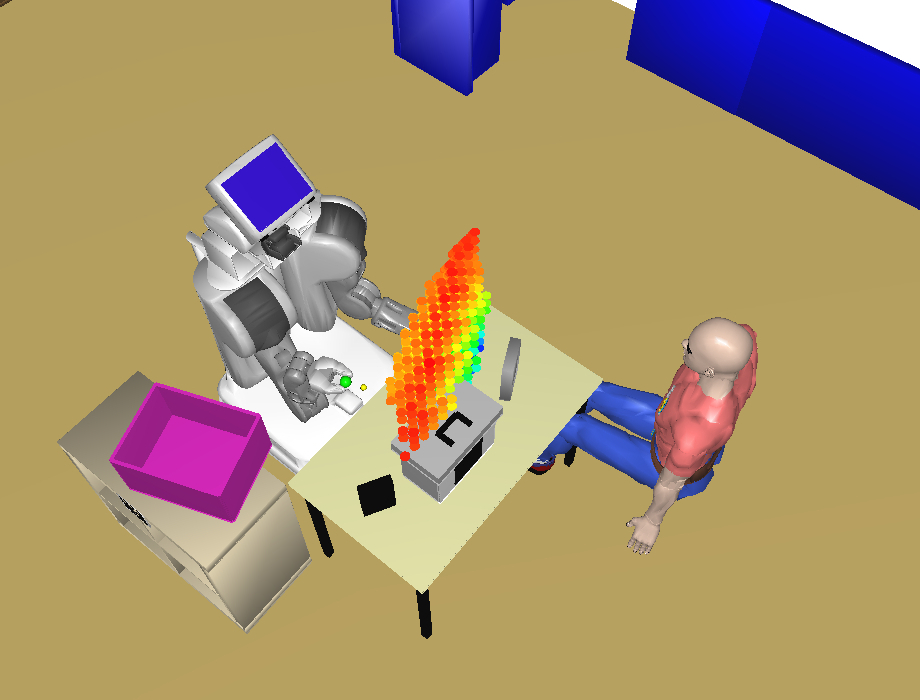
\includegraphics[width=0.5\textwidth]{./figs/mightabilities/4d.jpg}
       }
	\end{center}

   \caption{
	Steps for finding weighted candidate search space for the task of robot
	giving an object to the human.}
		
   \label{fig|mightabilities-steps}
\end{figure}



Figure~\ref{fig|mightabilities-steps} shows the main steps of finding the
candidate search space for the task of giving an object to the human by the
robot. From the initial set of all the MM for the robot and for the human, the
planner extracts the relevant MM based on the task and the desired efforts of
the agents.

In this example, the maximum desired effort for the human is to lean forward.
As the task requires a hand-over operation so the relevant MM obtained in step
(c) corresponds to the reach and visibility of both the agents, as shown in
figures~\ref{fig|mightabilities-steps}(a) and (b) for the robot and for the
human respectively.

Then the planner performs the set operations in step (d) to obtain the raw
candidate points in step (e). For the example task, the set operation is
finding the intersection of reachable and visible places by both the agents.
Figure~\ref{fig|mightabilities-steps}(c) shows the resultant candidate points
obtained in step (e), which in fact is commonly reachable and visible by both
the agents. 

Further based on various criteria such as comfort, preferences, etc. weights
are assigned to the raw candidate points in step (f) to obtain weighted
candidate points in step (g). Figure~\ref{fig|mightabilities-steps}(d) shows
the weighted candidate points, red cells are least preferable and green are
more preferable, so highest weight. At this step it is interesting to note that
the search space has been significantly reduced as compared to entire
workspace.  

In step (h) each candidate cell is iteratively tested for feasibility in the
order of highest to lowest weight until a solution is found. For finding a
feasible solution, various task-dependent constraints are introduced. Such
tests would have been very expensive if done for entire workspace.  In our
current implementation the first highest weighted candidate cell which
satisfies all the feasibility tests is accepted as the feasible solution of
highest weight, as shown in step (i). 

%Figure~\ref{fig|pr2-giving} show PR2 robot performing the task of giving an
%object to the human by finding the feasible solution through the presented
%framework. 
%
%
%\begin{figure}
%  \centering
%  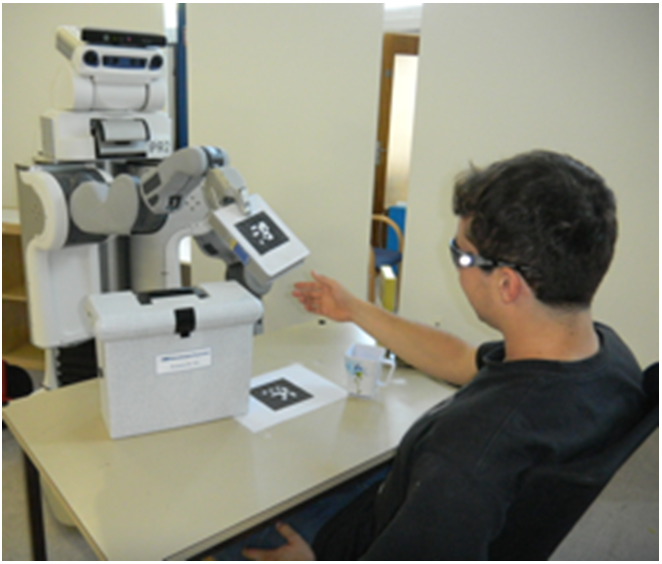
\includegraphics[width=0.8\textwidth]{./figs/mightabilities/5.png}
%  \caption { 
%PR2 giving an object to the human at a feasible place, which is easily visible
%and reachable by the human from his current position.
%}
%  \label{fig|pr2-giving}
%\end{figure}
%

\subsection{Related work}

Perspective Taking is a human ability which allows one to put
him/herself in another person's point of view. Studied in
psychology literature~\cite{Flavell1992,Tversky1999}, this ability is
crucial when interacting with people by allowing one to reason on
others' understanding of the world in terms of visual perception, spatial
descriptions, affordances and beliefs, etc.
Therefore, in the last years these notions have been gradually
employed in Human-Robot Interaction.~\cite{breazeal2006} presents a
learning algorithm that takes into account information about a
teacher's visual perspective in order to learn a
task. ~\cite{Johnson2005} apply visual perspective taking for action
recognition between two robots.~\cite{Trafton2005} use both visual and
spatial perspective taking for finding out the referent indicated by a
human partner.

%%%%%%%%%%%%%%%%%%%%%%%%%%%%%%%%%%%%%%%%%%%%%%%%%%%%%%%%%%%%%%%%%%%%%%%%%%%%
%%%%%%%%%%%%%%%%%%%%%%%%%%%%%%%%%%%%%%%%%%%%%%%%%%%%%%%%%%%%%%%%%%%%%%%%%%%%

\section{Explicit Knowledge Management}
\label{cognitivekernel}

\subsection{ORO: The OpenRobots Ontology server}

A key element of this cognitive architecture is how knowledge is explicitely
exposed, stored and handled between component.

We have adopted a centralized approach for knowledge management (while this is
the most commonly found approach in the litterature, other, more distributed
approaches exist, like \cite{Jacobsson2008}). Our knowledge base is called
ORO~\cite{Lemaignan2010}.

The ORO platform is primarily designed as a central
knowledge storage service implemented as a server where the robot
components can add or query statements at run-time. Figure~\ref{fig|oro-overview}
illustrates the overall architecture. The \emph{front-end} accepts and manages
connections from client components. The clients' requests are processed by a
set of internal modules: basic operations on statements, but also higher
cognitive and human-robot interaction related functionalities are available
(detailed thereafter). External plugins can also be easily added. The modules
rely on several parallel ontology \emph{back-ends} where the knowledge is
actually stored.

\begin{figure}[!t]
\centering
  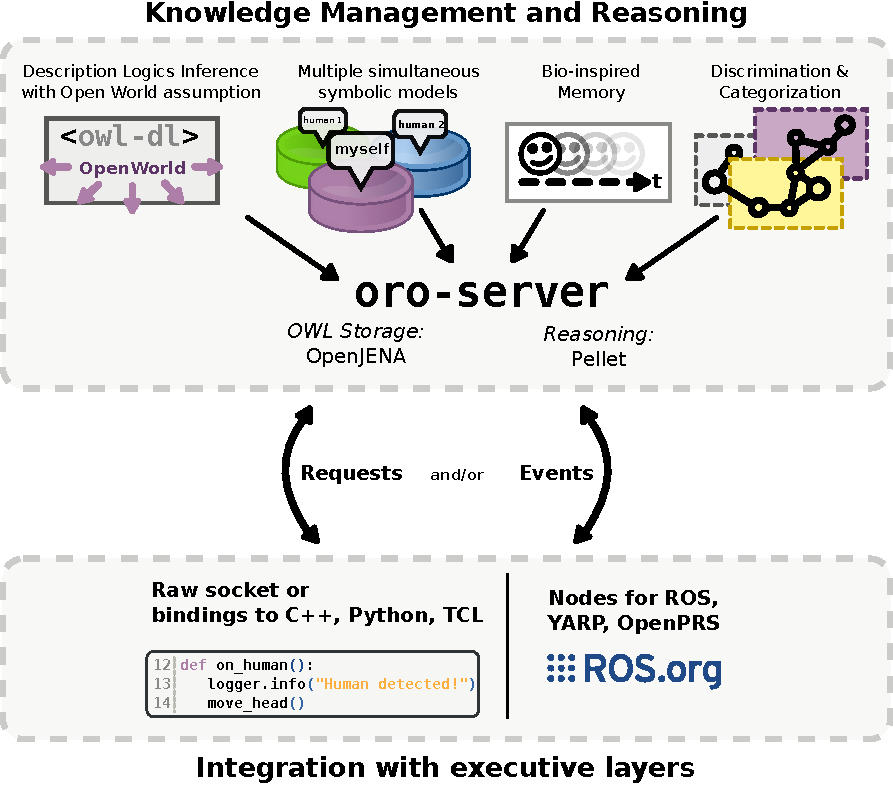
\includegraphics[width=0.8\linewidth]{figs/oro_architecture_functional.pdf}
  \caption{Overview of the ORO architecture.}
  \label{fig|oro-overview}
\end{figure}

Besides acting as a facts database, the ORO platform exposes several functions:
operations on knowledge statements relying on inference (through a continuous
first-order logic classification process), management of \emph{per-agent}
symbolic models, and also higher cognitive and human-robot interaction related
functionalities like categorization of sets of concepts, profiles of memory
(that enable the robot to ``forget'' about some facts), natural language
grounding~\cite{Lemaignan2011}\ldots.

ORO stores independent knowledge models (in our implementation, as
\emph{ontologies}) for each agent (the robot and the humans it
interacts with). The robot architecture components (like the executive
layer or the situation assessment component) can then store the
agents' beliefs in specific models.  Each of these models is
independent and logically consistent, enabling reasoning on different
perspectives of the world that would otherwise be considered as
globally inconsistent (for instance, an object can be visible for the
robot but not for the human. This object can have at the same time the
property \concept{isVisible \textbf{true}} and \concept{isVisible
  \textbf{false}} in two different models). This feature actually
allows us to consider the robot to be endowed with a simple
\emph{theory of mind}~\cite{Scassellati2002}: it can explicitly
model the belief state of its interactors.

ORO also provides an event mechanism that allows components to be
triggered when specific events occur. A component can
for instance subscribe to events of kind \setstmt{?agent isVisible
  true, ?agent type Human}. As soon as the perception layer detects a
human in the robot's field of view and accordingly updates the
knowledge base, the executive layer would be triggered back. The
event framework also takes advantage of the inference capabilities of
ORO. Thus an event can be indirectly triggered if its triggering
conditions can be inferred to be true.

\subsection{The OpenRobots Common-Sense Ontology}
\label{ontology}

For the robot to interpret and come up with new inferences based on the facts
coming from the perceptual layers, it need a \emph{cultural background}, a
common-sense knowledge assumed to be shared by all agents. The ORO server is
loaded at startup with an initial set of statements which we call the
\emph{OpenRobots Common Sense Ontology}. It defines a small set of concepts
(and implicitly, a vocabulary) that can be used by all the modules of the robot
to unambiguously add or query facts. Moreover, the same ontology declares rules
and logical properties that are later on used for inference.

The \emph{OpenRobots Common Sense Ontology} defines a small set of classes (56
are currently defined) and predicates (60 are currently defined) focused on
concepts useful for human-robot interaction. It includes both very broad
categories like \concept{SpatialThing}, \concept{Event} or \concept{Action},
and much more concrete concepts as \concept{Table}, \concept{Book} or colors.
Available predicates allow us to describe the state of the agents and the world
with relations like \concept{isOn}, \concept{sees},
\concept{currentlyPerforms}, etc.

Several significant projects are trying to provide such a machine-processable
repository of common sense facts produced by humans (the \textsc{OpenMind}
project\footnote{\url{http://www.openmind.org/}}, for instance). These
knowledge bases are valuable but remain difficult to use in a pervasive way
because of both their incompleteness and the lack of good connections with
underlying, unambiguous concepts.
%\cite{Singh2002}

Our common sense ontology is closely aligned with the open-source
OpenCyc\footnote{\url{http://www.opencyc.org}} upper ontology.
OpenCyc defines a large taxonomy of concepts and semantic
relationships between concepts that are used in several other projects
(\textsc{WordNet, DBpedia}). This potentially eases the exchange and addition
of knowledge from these other sources. Moreover, it also enables knowledge
exchange with other robots (for instance, the works previously mentioned by
Daoutis and Tenorth rely on the same Cyc concepts).

\subsection{Reasoning and Dynamic Knowledge Structuring}

As previously mentioned, ontologies in ORO are written in OWL. The
Pellet reasoner supports most of the OWL constructs and allows several types of
reasoning:

\begin{itemize}
	\item inheritance
	\item property axioms
		\begin{itemize}
		\item entailments based on predicates' domain and range,
		\item cardinality constraints (including \concept{allValue}, 
		\concept{someValue}, \concept{hasValue}),
		\item property characteristics (symmetry, transitivity)
		\end{itemize}
	\item class restrictions like: \par \footnotesize \concept{Bottle} $\equiv$
		\concept{Artifact} {\bf that} (\concept{hasShape} {\bf value}
		\concept{cylinderShape})\footnote{This example uses the \emph{Manchester
		syntax}, \url{http://www.w3.org/TR/owl2-manchester-syntax/}} \normalsize
	\item set operations like: \par \footnotesize \concept{Color} $\equiv$ {\bf unionOf}(\concept{blue},
		\concept{green}, \concept{orange}, \concept{black}...) \normalsize
	\item generic SWRL ({\em Semantic Web Rule Language}) rules like: \par
		\footnotesize \concept{looksAt(?agt, ?obj)} $\land$
		\concept{pointsAt(?agt,?obj)} \par $\Rightarrow$ \concept{focusesOn(?agt, ?obj)}
		\normalsize 
	\end{itemize}

We provide in ORO accessors to query, add or remove all these properties and
restrictions (except the SWRL rules) at run-time. This allows
knowledge introspection and enables the robot to alter its own knowledge
structures (the so-called \emph{T-Box} model) during its life-time by adding
new constraints and properties to classes and predicates.

\subsection{Representation of Alternative Cognitive Models}
\label{alterite}

As pictured in Figure~\ref{fig|oro-overview}, ORO stores independent cognitive
models for each agent it interacts with. When ORO actually identifies a new
agent (or infers that some instance is an agent), it automatically creates a
new, separate, in-memory OWL model for that agent. Thus, different robot
components, like supervision or situation assessment, may then store the
agents' beliefs in separate models. All knowledge processing functions in the
robot's primary model are equally available in every agent's model, which
allows us to store and reason on different (and possibly globally inconsistent)
models of the world.

Each of these models is independent and logically consistent,
enabling reasoning on different perspectives of the world that would otherwise
be considered as globally inconsistent (for instance, an object can be visible for the
robot but not for the human. This object can have at the same time the property
\concept{isVisible \textbf{true}} and \concept{isVisible \textbf{false}} in
two different models). 

This feature actually allows us to consider the robot to be endowed with a
\emph{theory of mind}~\cite{Scassellati2002}: the robot can explicitly model
the belief state of its interactors, opening new possibilities for the control
architecture. In section~\ref{exp:disambVPT} we present an example of how we use this feature to
make sense of user sentences from his/her point of view. Moreover,
these multiple models can be viewed as different interpretive scopes,
allowing the robot to interpret the same reality from different points of view.

% \subsection{Categorization}
% \label{categorization}
% 
% We have implemented several algorithms (common ancestors, computation of the
% best discriminant~\cite{Ros2010b}) to help the robot cluster a set of
% concepts based on their symbolic similarities. One particular application of these functions is discrimination.
% While interacting with a user, the robot quite often needs to clarify an
% ambiguity produced by its human partner. For instance, a user may refer to a
% ``bottle'' where two bottles are currently visible. Discrimination routines
% can identify possible (symbolic) differences (\eg the color or the size of the
% bottles) that permit the robot to ask an accurate question to the user in order
% to solve the ambiguity. This discrimination can occur from the robot's
% perspective or from a specific agent's perspective. Usage of these
% categorization abilities are illustrated in Sections~\ref{dialogs:disamb} and~\ref{spygame}.
% 


\subsection{Related work}

In the field of symbolic knowledge processing for robots, Gunderson and
Gunderson~\cite{Gunderson2008} introduce the concept of \emph{reification}
(based on both recognition and pre-afference) as an intermediate step between
pattern recognition and symbol grounding. Their underlying storage of knowledge
relies on ontologies and bio-inspired memory models. While sharing similar
foundations to our work, their proposal is based on fairly simple perceptual
modalities and does not develop complex symbolic models that could enable
human-robot interaction.

Suh et al.~\cite{Suh2007} develop {\sc OMRKF}, an ontology-based reasoning
framework for robotics. They tackle the grounding problem by storing low-level
facts (like SIFT visual features) in a layered symbolic architecture that works
well in simple sensori-motor spaces. However this approach raises concerns
regarding scalability and management of more complex entities or interactions.

Daoutis et al.~\cite{Daoutis2009} introduce one of the first complete
architectures for grounded human-robot interaction. They successfully bind
low-level percepts (including view-point independent SIFT based object
recognition) to a high-level knowledge representation and reasoning system.
They base their knowledge model directly on the \textit{ResearchCyc} ontology
(including the \textit{MicroTheories} concept), used in combination with the
{\sc CycL} language. This enables second-order logic modeling and access to a
large common-sense knowledge base.

Beetz et al.~\cite{Beetz2010} proposes a cognitive architecture called
\textsc{CRAM} (Cognitive Robot Abstract Machine) that integrates
\textsc{KnowRob}~\cite{Tenorth2009a}, a knowledge processing framework based on
Prolog. Its underlying storage is based on an OWL ontology, derived from
\textsc{OpenCyc}. \textsc{CRAM} and \textsc{KownRob} have been demonstrated on
several real-world scenarios, where natural language recipes extracted from
Internet had to be translated into plans and executed in a kitchen environment,
perceived and rebuilt on-line by the robots. While Prolog offers more flexible
modeling (no constraints on the arity of predicate, where Description Logics as
used in our work are limited to binary predicates), it is based on the closed
world assumption (if something cannot be inferred to be true, it is inferred to
be false) whereas we rely on the open world assumption, which is more realistic
in real world scenarios. A probabilistic extension of \textsc{KnowRob}, called
\textsc{ProbCog}~\cite{Jain2009} is also available. While in principle
possible, currently the CRAM architecture does not provide explicit support for
interacting with humans.

%%%%%%%%%%%%%%%%%%%%%%%%%%%%%%%%%%%%%%%%%%%%%%%%%%%%%%%%%%%%%%%%%%%%%%%%%%%%
%%%%%%%%%%%%%%%%%%%%%%%%%%%%%%%%%%%%%%%%%%%%%%%%%%%%%%%%%%%%%%%%%%%%%%%%%%%%

\section{First Application: Goal and Plan Management}
\label{sec|hatp}

\fxfatal[author=Severin]{Reformulate this section to put emphasis on 'How we
use the whole architecture to make symbolic planning grounded into the real
physical world.'}

The Goal and Plan Management activity involves the human-aware
symbolic task planner component and the dedicated robot controller
activity (Figure~\ref{architecture_fg}).

\subsection{Symbolic Task Planning}

In order to devise how a given goal can be accomplished, the robot has
to elaborate a plan,~\textit{i.e.} a set of actions to be achieved by
the robot and its human partners.  This is the role of a HATP
\cite{Alili2008} (for Human Aware Task Planner).  HATP is based on a
Hierarchical Task Network (HTN) refinement which performs an iterative
task decomposition into sub-tasks until reaching atomic
actions~\cite{Nau2003}.  The planning domain defines a set of methods
describing how to decompose a task and can be seen as the Howto
knowledge of the robot.  HATP is able to produce plans for the robot's
actions as well as for the other participants (humans or robots). It
can be tuned by setting up different costs depending on the actions to
apply and by taking into account a set of constraints called social
rules. This tuning aims at adapting the robot's behavior according to
the desired level of cooperation of the robot.

%\subsubsection*{Agents and action streams:}
\vspace{0.3cm}
\noindent
\textbf{Agents and action streams:}
The robot plans not only for itself but also for the other agents. The
resulting plan, called ``shared plan'' is a set of actions that form
a stream for each agent involved in the goal achievement. Depending on
the context, some ``shared plans'' contain causal relations between
agents. For example, the second agent needs to wait for the success of
the first agent's action to be able to start its own action. When the
plan is performed, causal links induce synchronization between
agents. Figure~\ref{plan_hatp1} illustrates a plan with two streams.

\begin{figure}[htbp]
  \centering
  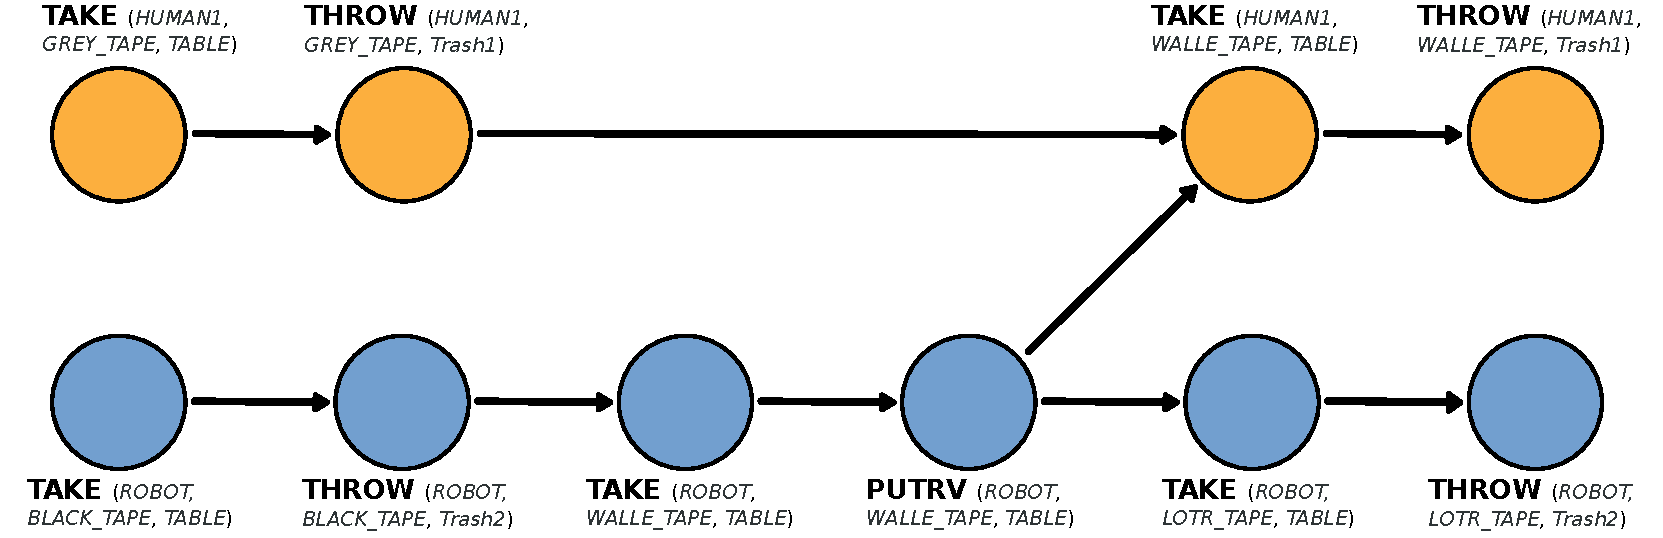
\includegraphics[width=0.95\columnwidth]{./figs/plan1.pdf}
  \caption{A plan produced by HATP with 2 streams}
  \label{plan_hatp1}
\end{figure}

\subsubsection{Action costs and social rules:}
A cost and a duration function is associated to each action.
The duration function provides a duration interval for the action
achievement and is used, in one hand, to schedule the different
streams and, in the other hand, as an additional cost function.
In addition to these costs, HATP also takes into account a set of social
rules.  Social rules are constraints aiming at leading the plan
construction towards the best plan according to some human
preferences. The social rules we have defined so far deal with:

\begin{itemize}
\item undesirable state: to avoid a state in which the human could
  feel uncomfortable;
\item undesirable sequence: to eliminate sequences of actions that can
  be misinterpreted by the human;
\item effort balancing: to adjust the work effort of the agents;
\item wasted time: used to avoid long delays between the actions of
  the human partner;
\item intricate links: to limit dependencies between the actions of
  two or more agents.
\end{itemize}

\begin{figure}[htbp]
  \centering
  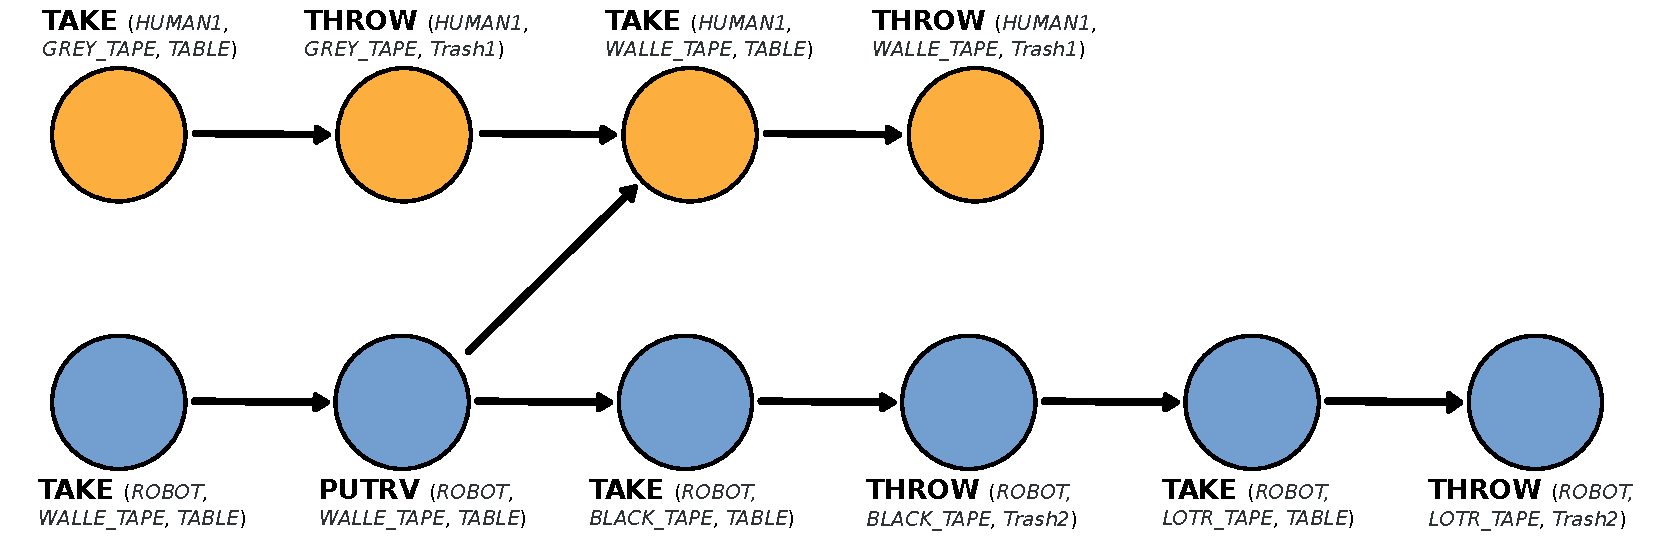
\includegraphics[width=0.95\columnwidth]{./figs/plan2.pdf}
  \caption{A plan with the wasted time social rule}
  \label{plan_hatp2}
\end{figure}

Figure~\ref{plan_hatp2} illustrates an alternative plan to the previous 
one (Figure~\ref{plan_hatp1}) if the wasted time social rule is used.
The obtained shared plan is the best plan according to a global evaluation of
these multiple criteria.

\subsubsection{Several levels of cooperation:} 

By tuning its costs
and adapting its social rules, HATP can be used to compute various
alternative plans. These plans can be categorized into several levels
of cooperation

\begin{itemize}
\item helping the human to achieve his goal by acting for him
\item sharing concrete resources by handing some objects
\item collaboration of the robot and the human by coordinating their
  actions towards a human-robot joint goal.
\end{itemize}




%%%%%%%%%%%%%%%%%%%%%%%%%%%%%%%%%%%%%%%%%%%%%%%%%%%%%%%%%%%%%%%%%%%%%%%%%%%%
%%%%%%%%%%%%%%%%%%%%%%%%%%%%%%%%%%%%%%%%%%%%%%%%%%%%%%%%%%%%%%%%%%%%%%%%%%%%

\section{Second Application: Natural Language Grounding}
\label{dialogs}

Looking back at our initial example, we wanted to make sense of the utterance
``\emph{Robot, put the two glasses and this bottle on the tray!}''.

The first step is to understand the meaning of the sentence. To this end, we
must acquire the sentence, convert it into a useful syntactic form (probably
through speech recognition), and understand the semantics of the sentence, \ie
What is referred by ``\textit{Robot}''? What is ``\textit{put}''? What are
``\textit{the}''? And ``\textit{two}''? etc.

Working in a situated context, we need to \emph{resolve} these semantics atoms,
\ie group them and then, ground them in the sensory-motor space of the robot. For instance,
``\textit{this bottle}'' is a demonstrative group that refers in this context to the
bottle the human is focusing on.

The next step is to extract and understand the \emph{intended meaning} of the
utterance as thought by the agent. In our example, Tom obviously wants an
action to be performed by the robot. The action parametrization is conveyed by
the semantics attached to the words and the grammatical structure of the
sentence. In our example, the type of action is given by the verb
``\textit{put}''. Assuming the robot has some procedural knowledge attached to
this symbol, the action type can be considered as grounded for the robot. We
can as well understand that the recipient of the action is the human, the
performer is the robot itself, and the objects acted upon are two glasses and a bottle. The
recipient, performer and object are three of the \emph{thematic
roles}~\cite{Gruber1965} that qualify the \emph{put} action. They are
necessary to fully ground the sentence\footnote{This analysis has been inspired
on the work of Austin et al.~\cite{Austin1962}, where this type of sentences
correspond to \emph{speech acts}, comprising of \emph{locutionary act} (the
meaning), \emph{illocutionary} (the intent) and possibly \emph{perlocutionary
acts} (implicit speaker's expectation).}.

To summarize, verbal interaction with human presents two categories of challenges: syntactic
ones, and semantic ones. The robot must be able to process and analyze the
structure of human utterances, \ie natural language sentences, and then make
sense of them. 

In this second application of our cognitive architecture, we show how we
harness the symbolic knowledge base to ground, interpret and act on verbal
instructions.

Furthermore, this process takes full advantage of the embodied nature of the
interaction: because deictic gestures and postures are also available in the
symbolic knowledge base (as presented in section~\ref{spark-deitic}) and
dynamically updated during the interactions, verbal dialogue processing turns
into a truely multi-modal communication processing, leading to more robust
interpretation.

We present here the processing of three categories of sentences:
\emph{statements}, \emph{desires} and \emph{questions} that can be answered
from the declarative knowledge present in the robot knowledge base (a choice
similar to the \emph{Behaviour Cycle} in the GLAIR
architecture~\cite{Shapiro2009}). In our work, the grounding process of the
human discourse consists in extracting either the \emph{informational} content
of the sentence to produce statements or its \emph{intentional} content (\ie
performative value) to collect orders and questions. We focus this application on the grounding (we call it
\emph{resolution}) of concepts involved in the human discourse through the
robot's own knowledge: refer to Kruijff et al.~\cite{Kruijff2010}
for a broader survey of formal approaches to natural language processing in the
robotics field.

\begin{figure}[!t]
\centering
  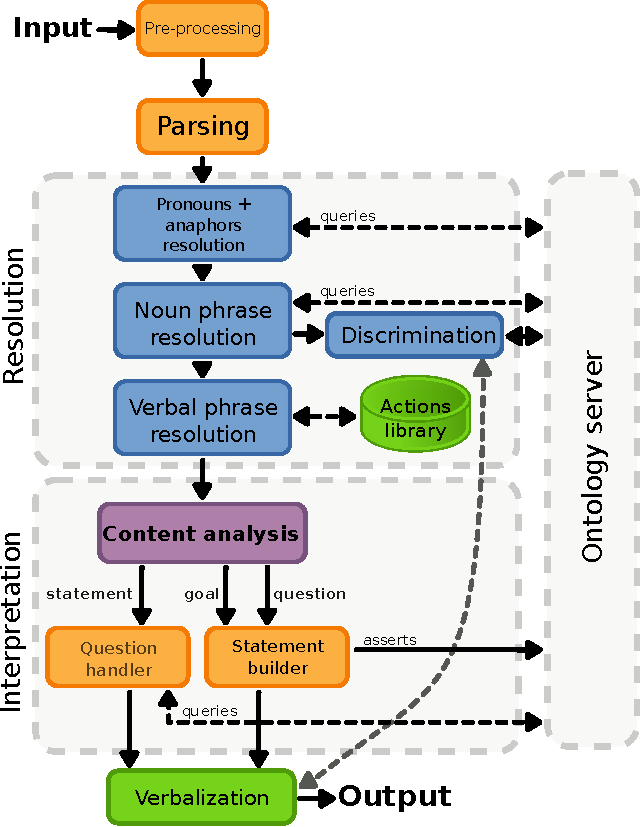
\includegraphics[width=0.7\linewidth]{figs/dialog_module_simple.pdf}
  \caption{The {\sc Dialogs} module has three main steps: the parsing,
  the interpretation and the verbalization. The interpretation module is
  responsible for both the \emph{resolution} and the semantic content
  \emph{analysis and translation}.} 
  \label{fig|dialog}
\end{figure}

Our dialogue processing is done by a module called {\sc Dialogs} (Figure~\ref{fig|dialog}) that processes human
input in natural language, grounds the concepts in the robot's knowledge and
eventually translates the discourse in a set of queries or declarative OWL/RDF
statements.  

The user's input is first pre-processed. For instance, \emph{I'm} constructs are expanded
into \emph{I am} and then parsed by a rule-based (\ie
grammar-free) tool that extracts the grammatical structure from the user's
sentence. Figure~\ref{dialog|parser_output} shows an example of the raw output of the parser for a moderately complex sentence.

\begin{figure}%[!ht]
\begin{center}
\scriptsize
\begin{alltt}
>> IMPERATIVE
VP: \textbf{remember} (present simple)
    SUBSENTENCE (aim: that)
      NP: \textbf{I}
      VP: \textbf{want} (present simple)
        direct objects: 
          NP: \textbf{you}
        secondary VP: \textbf{give} ()
              direct objects:
                NP: my \emph{nice blue} \textbf{bottle}
              indirect objects:
                NP: \textbf{me}
\end{alltt}
\end{center}
\caption{Raw output of the {\sc Dialogs} parser after processing the
sentence: ``remember that I want you to give me my nice blue bottle.'' 
Nominal groups are not grounded yet.} 
\label{dialog|parser_output}
\end{figure}

The output of the parser is then sent to the \emph{interpretation} module, the
core of the component.  Interpretation consists in three distinct operations:
the sentence \emph{resolution} (concepts grounding), the \emph{content
analysis} (what is the intent of the utterance: information, question or
desire) and the \emph{statement building} (translation into RDF statements).

The sentence resolution has three steps: {\it(i)} pronouns and anaphora are
replaced by the correct speaker ID and the ID of the last object referred to
(extracted from the dialogue history) respectively, {\it(ii)} nominal groups are
disambiguated and grounded (noun phrase resolution), and {\it(iii)}
verbal groups are resolved and their associated \emph{thematic roles} are
retrieved (verb phrase resolution).

\small
\begin{pseudocode}[ruled]{Resolution}{sentence, currentSpeaker}
\label{algo|Resolution}

\mathcal{G} \GETS \CALL{ParseNominalGroups}{sentence} \\

\FOREACH g \in \mathcal{G} \DO 
\BEGIN
   \mathcal{D} \GETS \CALL{GenerateDescription}{g} \STMTNUM{5.1em}{res.desc}\\
   candidates \GETS \CALL{Ontology.Find}{\mathcal{D}} \STMTNUM{4em}{res.onto}\\
   
   \IF \left|{candidates}\right| = 0 \THEN
    \BEGIN
      \OUTPUT{\mbox{Couldn't resolve the group!}} \\
      \EXIT \\
    \END
   \ELSEIF \left|{candidates}\right| = 1 \THEN
      id \GETS candidates[0]\\

   \ELSE
      \BEGIN
	\IF \CALL{Ontology.CheckEquivalent}{candidates} \THEN
	  id \GETS candidates[0] \\
	\ELSE
	  id \GETS \CALL{Discrimination}{candidates} \STMTNUM{0em}{st.discrimination}\\
      \END \\
   \CALL{Replace}{g, id, sentence}
\END
\end{pseudocode}
\normalsize

As represented in Figure~\ref{fig|dialog}, interpretation tightly relies on the
communication with the knowledge base. All the concepts the robot manipulates
are stored in the ontology server and retrieved through logical
queries, except for the verbs that are currently stored in a dedicated library
(the \emph{action library} in the diagram).

%%%%%%%%%%%%%%%%%%%%%%%%%%%%%%%%%%%%%
%\section{Technical analysis}
%\label{examples}

In order to better understand the overall process of the {\sc Dialogs} module 
and its relation with ORO, we next describe the different steps of the approach 
based on three examples. In these examples we assume that some initial facts 
are present in the knowledge base (section~\ref{modeling_real_world} discusses how 
the initial knowledge can be acquired), both in the robot's own model and in the human's model.  Since the robot tries to ground a human utterance, all queries are sent to the human model in order to interpret it from the human perspective. 

\subsection{Informational Content Extraction}
\label{informational_content_extraction}

%\begin{figure}
%    \centering
%	\begin{tabular}{p{7cm}}
%	\emph{Initial knowledge model of} \texttt{human\_01}\\
%	\hline
%    	\hspace{0.3cm}\stmt{banana\_01 type Banana} \\
%    	\hspace{0.3cm}\stmt{banana\_01 hasColor yellow}\\
%	
%	\vspace{0.5em}
%	\emph{Human input}\\
%	\hline
%	\hspace{0.3cm}``The yellow banana is big!'' \\
%
%	\vspace{0.5em}
%	\emph{Generated partial statements}\\
%	\hline
%	\hspace{0.3cm}\stmt{?obj type Banana} \\
%    	\hspace{0.3cm}\stmt{?obj hasColor yellow} \\
%    	\hspace{0.7cm}$\Rightarrow$ \concept{?obj = banana\_01}\\
%
%	\vspace{0.5em}
%	\emph{Newly created statements}\\
%	\hline
%	\hspace{0.3cm}\stmt{banana\_01 hasSize big} \\
%	\end{tabular}
%\caption{First example of natural language grounding: the nominal group ``the
%yellow banana'' is matched with the individual \concept{banana\_01}.
%``$\Rightarrow$'' represents the output of the ontology server.}
%\label{dialog|ex1}
%\end{figure}

\begin{figure}
    \centering
%	\begin{tabular}{p{0.5\columnwidth} | p{0.5\columnwidth}}}
	\begin{tabular}{l|l}
	\emph{Initial knowledge} \texttt{human\_01} &
	\emph{Human input}\\	
	
	\hline

    	\stmt{banana\_01 type Banana} &
	``The yellow banana is big!'' \\
	
    	\stmt{banana\_01 hasColor yellow} & \\
	\vspace{0.5em}\\
	\hline

	\emph{Generated partial statements} &
	\emph{Newly created statements}\\
	\hline

	\stmt{?obj type Banana} &
	\hspace{0.2cm}\stmt{banana\_01 hasSize big} \\
	
    	\stmt{?obj hasColor yellow} & \\
    	\hspace{0.2cm}$\Rightarrow$ \concept{?obj = banana\_01}\\

	\hline
	\end{tabular}
\caption{First example: content extraction.
``$\Rightarrow$'' represents the output of the ontology server.}
\label{dialog|ex1}
\end{figure}


Figure~\ref{dialog|ex1} shows a first example of human discourse grounding and
the extraction of informational content. We assume that the robot knowledge
base only contains two initial statements in the human model. The user
asserts a new one: ``The yellow banana is big!''. 
We first want to match the nominal group \emph{The yellow banana} to an already
known concept (algorithm~\ref{algo|Resolution}), and second to translate the property \emph{is big} into a predicate ({\tt hasSize}) to state its semantics. 

To resolve the nominal group \emph{The yellow banana} a set of partial
statements that describe the concept is generated based on the grammatical
parsing of the sentence (algorithm~\ref{algo|Resolution}(\ref{res.desc})). The parsed tree of each nominal group is translated into statements based on a set of rules.
In the example, a banana (\stmt{?obj type Banana})
that is yellow (\stmt{?obj hasColor yellow})\footnote{Predicates like
\concept{hasColor} or \concept{hasSize} that bind \concept{banana\_01} to
adjectives are extracted from a predefined database of $[Predicate \rightarrow
AdjectiveCategory]$, and falls back on the generic \concept{hasFeature}
predicate if the adjective is not known.}.  Based on these partial statements a
SPARQL query is sent to the ontology server to retrieve possible instances that match
the description (algorithm~\ref{algo|Resolution}(\ref{res.onto})).

In this first simple case, the concept \concept{banana\_01} is unambiguously
matched (since there is only one possible banana) and returned. Finally, we can
now add the new information provided by the human, \ie the new statement
\stmt{banana\_01 hasSize big}, to the human model in the ontology server.

% The translation of \emph{yellow} to \stmt{hasColor yellow} is not obvious: in
% the general case, we associate a adjective to the noun it characterizes with
% the \concept{hasFeature} predicate (for instance, \emph{The sight is beautiful}
% would translate to \stmt{sight hasFeature beautiful}). But we can also manually
% set the predicate associated to a category of adjectives: It is what has been
% done for the main colours. Another example is the size: for known size
% adjectives (big, small, etc.), the \concept{hasSize} predicate is being used.


\subsection{Intentional Content Through Verb Resolution}
The sentence in the first example is built with the state verb \emph{be} at
indicative. Let us examine a different example with an action verb at
imperative mode (an order): ``Give me the banana". The process is
described in Figure~\ref{dialog|ex2}.

%\begin{figure}
%    \centering
%	\begin{tabular}{p{7cm}}
%	\emph{Initial knowledge model of} \texttt{human\_01}\\
%	\hline
%    	\hspace{0.3cm}\stmt{banana\_01 type Banana} \\
%    	\hspace{0.3cm}\stmt{banana\_01 hasColor yellow}\\
%	\end{tabular} \\
%
%	\vspace{0.5em}
%
%	\begin{tabular}{p{7cm}}
%	\emph{Human input}\\
%	\hline
%    	\hspace{0.3cm}``Give me the banana.'' \\
%	\end{tabular} \\
%
%	\vspace{0.5em}
%
%	\begin{tabular}{p{7cm}}
%	\emph{Generated partial statements}\\
%	\hline
%    	\hspace{0.3cm}\stmt{?obj type Banana} \\
%	\hspace{0.7cm}$\Rightarrow$ \concept{?obj = banana\_01}\\
%
%	\end{tabular} \\
%
%	\vspace{0.5em}
%
%	\begin{tabular}{p{7cm}}
%	\emph{Newly created statements}\\
%	\hline
%    	\hspace{0.3cm}\stmt{human\_01 desires situation\_a3f74} \\
%    	\hspace{0.3cm}\stmt{situation\_a3f74 type Give} \\
%    	\hspace{0.3cm}\stmt{situation\_a3f74 performedBy myself} \\
%    	\hspace{0.3cm}\stmt{situation\_a3f74 actsOnObject banana\_01} \\
%    	\hspace{0.3cm}\stmt{situation\_a3f74 receivedBy human\_01} \\
%	\end{tabular}
%
%\caption{Second example: processing an order.}
%\label{dialog|ex2}
%\end{figure}

\begin{figure}
    \centering
	\begin{tabular}{l|l}
	\emph{Initial knowledge} \texttt{human\_01} &
	\emph{Human input}\\
	
	\hline
	
    	\stmt{banana\_01 type Banana} &
	``Give me the banana.'' \\
	
    	\stmt{banana\_01 hasColor yellow} & \\
	\vspace{0.5em}\\
	\hline
    	
	\emph{Generated partial statements} &
	\emph{Newly created statements}\\
	\hline
    	\stmt{?obj type Banana} & 
	\stmt{human\_01 desires sit\_a3} \\
	
	\hspace{0.2cm}$\Rightarrow$ \concept{?obj = banana\_01}
    	& \stmt{sit\_a3 performedBy myself} \\
    	& \stmt{sit\_a3 actsOnObject banana\_01} \\
    	& \stmt{sit\_a3 receivedBy human\_01} \\
	\end{tabular}

\caption{Second example: processing an order.}
\label{dialog|ex2}
\end{figure}


\label{processing_of_actions}

In order to capture the intentional content of a sentence (for example, an
order) we need to retain the semantics of the verb and its complements.
\emph{Thematic roles} allow for semantically linking a verb to its complements.  
There is no general agreement amongst linguists on a comprehensive list of 
thematic roles. The amount and the granularity of roles varies a lot in 
the literature~\cite{Gutierrez2001}. We thus use a small set of them, which matches
the relations the robot can actually achieve (we discuss
possible extensions in the conclusion). For instance, in the second example,
the verb \emph{give} has three thematic roles: \concept{performedBy},
\concept{actsOnObject} and \concept{receivedBy}.

The list of actions the robot can plan for (currently \emph{take},
\emph{place}, \emph{give}, \emph{show}, \emph{hide} and \emph{move}) along with
possible synonyms (for example, \emph{to pick} is set as a synonym of \emph{to
take}) and their associated thematic roles are stored in a predefined library
of actions. For each action we identify and store: the role of the subject in
the sentence (always \concept{performedBy}); the role of the direct object
(for instance, \concept{actsOnObject}); and the role of each of the indirect
objects with their optional prepositions (for instance,
\concept{receivedBy})\footnote{Note that in example 2, ``give me the banana'',
the pronoun ``me'' appears before ``banana'', while it is an indirect
complement --- ``give it {\bf to me}''. The parser correctly handles these
cases.}. Moreover, through the ontology we check that each holder of a
role is semantically consistent. For instance, the action \emph{Give} must have a
manipulable physical item (\concept{Artifact}) as direct object. Thus, if the
concept the robot finds for the thematic role \concept{actsOnObject} cannot be
inferred to be an artifact, the robot goes back to the human saying it does not
understand.

This second example  also shows the pronoun reference resolution: ``me'' is
replaced by the id of the current speaker, while ``you'' is replaced by
\concept{myself} (\concept{myself} always represents the robot itself). When
present, anaphoras (references to previous concepts like ``give me the banana, I
like {\bf it}.'') are also resolved in the same step.

Once the sentence is completely resolved and translated into a formal
representation (a human desire in this example\footnote{Orders are here
represented as human desires: the human desires a specific new situation.}), we
store it in the ontology server. The robot's decisional/executive layers can
then decide whether to execute the order or not. 

\subsection{Informational Content Extraction Requiring Clarification}
\label{dialogs:disamb}
\begin{figure}
    \centering
	\begin{tabular}{p{7cm}}
	\emph{Initial knowledge model of} \texttt{human\_01}\\
	\hline
     	\hspace{0.3cm}\stmt{banana\_01 type Banana} \\
     	\hspace{0.3cm}\stmt{banana\_01 hasColor yellow} \\
     	\hspace{0.3cm}\stmt{banana\_02 type Banana} \\
     	\hspace{0.3cm}\stmt{banana\_02 hasColor green} \\
	\end{tabular} \\

	\vspace{0.5em}

	\begin{tabular}{p{7cm}}
	\emph{Human input}\\
	\hline
     	\hspace{0.3cm}``The banana is good.'' \\
	\end{tabular} \\

	\vspace{0.5em}

	\begin{tabular}{p{7cm}}
	\emph{Generated partial statements}\\
	\hline
     	\hspace{0.3cm}\stmt{?obj type Banana} \\
	\hspace{0.7cm} $\Rightarrow$ \concept{?obj = [banana\_01, banana\_02]}
	\end{tabular} \\

	\vspace{0.5em}

	\begin{tabular}{p{7cm}}
	\emph{Discrimination process}\\
	\hline
     	\hspace{0.3cm}\concept{discriminate([banana\_01, banana\_02])} \\
	\hspace{0.7cm} $\Rightarrow$ \concept{?hasColor = [yellow, green]}
	\end{tabular} \\

	\vspace{0.5em}

	\begin{tabular}{p{7cm}}
	\emph{Robot output speech}\\
	\hline
     	\hspace{0.3cm}``The yellow one or the green one?'' \\
	\end{tabular} \\

	\vspace{0.5em}

	\begin{tabular}{p{7cm}}
	\emph{Human answer}\\
	\hline
     	\hspace{0.3cm}``The green one.'' \\
	\end{tabular} \\
    
	\vspace{0.5em}

	\begin{tabular}{p{7cm}}
	\emph{Extended human input}\\
	\hline
     	\hspace{0.3cm}``The green banana is good.'' \\
	\end{tabular} \\
	
	\vspace{0.5em}

	\begin{tabular}{p{7cm}}
	\emph{Generated partial statements}\\
	\hline
     	\hspace{0.3cm}\stmt{?obj type Banana} \\
     	\hspace{0.3cm}\stmt{?obj hasColor green} \\
	\hspace{0.7cm} $\Rightarrow$ \concept{?obj = [banana\_02]}
	\end{tabular} \\
    
	\vspace{0.5em}
	\begin{tabular}{p{7cm}}
	\emph{Newly created statements}\\
	\hline
     	\hspace{0.3cm}\stmt{banana\_02 hasFeature good} \\
	\end{tabular}

\caption{Ambiguity resolution: in this example, ``banana'' can refer to the
yellow banana (\concept{banana\_01}) or the green one (\concept{banana\_02}).
Discrimination routines handle the disambiguation process.} \label{dialog|ex3}
\end{figure}

This last example (Figure~\ref{dialog|ex3}) shows the resolution of ambiguous
concepts. In this case the user refers to ``the banana'' while two instances of 
the \concept{Banana} class exist in the ontology. The robot needs to find out
to which instance the user is actually referring to. To this end,
disambiguation routines (algorithm~\ref{algo|Resolution}(\ref{st.discrimination}), see \cite{Ros2010b} for details of the routines)
find differences between the instances (in the example, one banana is yellow
while the other one is green) and build a sentence through the
\emph{verbalization} module to ask the user a closed question that will
help clarify the ambiguity: ``Is it yellow or green?'' The user's answer is
parsed and merged with the previous sentence. The resulting, augmented,
sentence (``The green banana is good") goes again through all the
interpretation steps. This process is repeated until no ambiguities arise. 
In the example, the \concept{banana\_02} is finally returned.

%If no differences \fxfatal{should we say 'in the human model', even if 
%getDiscriminantForAgent currently doesn't work?} can be found, an open question 
%(``give me more information'') is send to the human.

Several other strategies are used in parallel to disambiguate concepts without
having to ask for more information to the human:

\begin{itemize}
	\item Which objects are currently visible to the human? If only one of
	them, then it is probably the one the user is talking about. 
	\item Did a previous interaction involved a specific object that would
	still be the subject of the current sentence?
	\item Is the user looking or pointing at a specific object?
\end{itemize}

%Two cases can alter the way the discrimination routines work:
%\begin{enumerate}
%    \item If a sentence starts with {\it Learn that...}, failures during 
%    discrimination are interpreted as new concepts, and instead of marking the 
%    nominal as not resolved, and new identifier is created and add to the knowledge base.
%    \item For questions like {\it Which color is the bottle?}, the discrimination 
%    algorithm can not use the feature {\it color} to identify to bottle. The 
%    resolution algorithm pass this kind of constraints as a parameter of the 
%    discrimination routines.
%\end{enumerate}

 
While no examples involving questions have been detailed, factual \emph{wh-}
questions and polar (\emph{yes/no}) questions can be processed in a similar way
by \textsc{Dialogs}. For instance, a question like ``What is on the table?'' is
grounded (to extract the relation \concept{isOn} and to find what \emph{table}
refers to) and transformed into the following kind of query: \concept{find ?var
[\stmt{?var isOn table1}]}.  Answers are converted back to a full sentence by
the \emph{verbalization} module, and uttered to the human.

\subsection{Related work}

Processing natural language in situated contexts is already an established
research field. In~\cite{Roy2005}, Roy and Reiter summarize what they see as
the main challenges to be tackled: cross-modal representation systems,
association of words with perceptual and action categories, modeling of
context, figuring out the right granularity of models, integrating temporal
modeling and planning, ability to match past (learned) experiences with the
current interaction and ability to take into account the human perspective.
This list offers an interesting entry point to evaluate our contribution.

Kruijff et al. provides in~\cite{Kruijff2010} an up-to-date survey of
literature on situated human-robot dialogue, focusing on formal representation
systems, bi-directionality of the interaction and context building. They point
out as well that compared to the cognitive psychology community, the ``situated
AI'' community started only recently to take into account agents' focus of
attention, perspective and temporal projection abilities.

Dialogue processing in real robots have been explored by several teams.  Brick
and Scheutz~\cite{Brick2007} have contributions regarding natural language
processing in an incremental way, and how this enables instant back-channel
feedback (like nodding). Hüwel et al.~\cite{Huwel2006} propose the concept of
\textit{Situated Semantic Unit}: atoms are extracted from sentences exposing
semantic links to other units. The parser tries to satisfy these links and
rates the semantic interpretation of the sentence. Used in conjunction with
ontologies, their approach offers robustness to ungrammatical or partial
utterances. They validated the approach with an extensive user-study.

Zender et al.~\cite{Zender2009} address the generation of referring expressions
(GRE~\cite{Dale1995}) in situated dialogue for topological knowledge.  They consider
both the reference resolution and reference description tasks, and rely on
OWL-DL representation and SPARQL\footnote{{\em SPARQL Protocol and RDF Query
Language}, \url{http://www.w3.org/TR/rdf-sparql-query/}} to extract
\emph{topological contexts} from their knowledge base.

%%%%%%%%%%%%%%%%%%%%%%%%%%%%%%%%%%%%%%%%%%%%%%%%%%%%%%%%%%%%%%%%%%%%%%%%%% 
%%%%%%%%%%%%%%%%%%%%%%%%%%%%%%%%%%%%%%%%%%%%%%%%%%%%%%%%%%%%%%%%%%%%%%%%%% 

\section{Conclusion}
\label{conclusion}

\subsection{Grounding the Human Interaction: Specifics and Alternative Approaches}

Before concluding the chapter, this section gives some pointers to the specifics of the human-robot interaction context, 
and to other contributions implementing alternative grounding strategies in such a context.


The human presence brings specific requirements for robot's abilities both
at the functional and at the deliberative levels~\cite{Klein2004}. This touches several domains:
 motion~\cite{Kulic2007,Berg2004,Madhav2006},
navigation~\cite{Althaus2004,Sisbot2007}, manipulation~\cite{Kemp2007}
in presence of humans as well as perception of human
activities~\cite{Breazeal2001,Burger2008}.

Also, when interacting with humans, robots need to incorporate communication and
collaboration abilities. Several theories dealing with
collaboration~\cite{Cohen1991,Grosz1996,Clark1996} emphasize that
collaborative tasks have specific requirements compared to individual
ones, \eg, since the robot and the person share a common goal, they
have to agree on the manner to realize it, they must show their
commitment to the goal during execution, etc. Several robotic systems
have already been built based on these theories~\cite{Rich1997,Sidner2005,Tambe1997,Breazeal2003} and they
all have shown benefits of this approach. They have also shown how
difficult it is to manage turn-taking between communication partners
and to interleave task realization and communication in a generic
way. Finally, today only few systems~\cite{Fong2006,Breazeal2003,Sisbot2008} take humans into
account at all levels.

\fxwarning{If relevant, describe Breazeal approaches for grounding}

While mostly implemented on virtual agents, the GLAIR cognitive architecture by
Shapiro and Bona~\cite{Shapiro2009} is an architecture explicitly built to
tackle the grounding issue from the percept to the decision. It is a
three-layers architecture: a \emph{Knowledge Layer}, a low-level
\emph{Sensori-Actuator Layer} and an intermediate \emph{Perceptuo-Motor Layer}
that binds the previous two.  The knowledge layer relies on a custom knowledge
representation language (more expressive than first-order logic), and natural
language processing capabilities similar to ours are available. The GLAIR
project has been only demonstrated in a limited set of environments, but
exhibits interesting features such as explicit management of contexts of facts
and memory models (long term/short term, episodic/semantic).

Also worth mentioning, Mavridis and Roy~\cite{Mavridis2005} propose the idea of
a \emph{grounded situation model} which is an amodal model of the world where
different sensing modalities, including verbal ones (the robot is able to
\emph{imagine} objects), are merged. Their framework also allows the management of
the interaction history (the human can ask for a past event). They propose an
implementation in an environment built on simple entities (a manipulator arm
and colored balls).



\subsection{Towards an Event-Driven, Knowledge-Oriented Architecture for Personal Robotics}

In this paper, we have studied knowledge streams between three components: {\it(1)}
{\sc ORO}, an ontology-based knowledge server that stores and maintains
classified RDF statements produced by other modules in agent-specific
models and allows information to be easily retrieved, either through queries or
via an event system; {\it(2)} {\sc SPARK}, the grounded, human-aware 3D model
of the environment that performs all the spatial reasoning within our
architecture, including reasoning involving motion planing (to compute
reachability of objects) and perspective taking, and {\it(3)} {\sc Dialogs}, a
natural language processor that performs simple grammatical parsing of English
language, grounds the semantic content of the utterance (if necessary, also
interacts with the user to disambiguate), and eventually generates a RDF
representation of the sentence.

These components, combined with modules dedicated to symbolic supervision and
task planning (these modules are outside of the scope of this article), compose
an architecture that we call \emph{knowledge-oriented}:

\begin{itemize}
\item{Knowledge is explicitly stored in one central and consistent repository
of facts, accessible by all modules.}
\item{Knowledge is represented in a strict formalism (OWL statements) and
with a clearly defined vocabulary (stated in the {\tt commonsense.oro.owl}
ontology).}
\item{The first two points enable both a loosely-coupled
architecture where modules can very easily be removed or replaced by other ones
as long as they share the same semantics (modules are defined by the knowledge
they produce),}
\item{and a \emph{symbolic} reactive, event-driven approach
to supervision. By managing events at the same level as
the reasoner, we take full advantage of the inference abilities of ORO to
trigger events whose \texttt{true} conditions can be inferred.}
\item{Finally, this architecture allows for the combination of very different knowledge
modalities in a single homogeneous environment, bringing mutual benefits to
components. For instance, the dialogue processing module can perfectly run
without any geometric perception, but its disambiguation routines can
transparently benefit from it when available (since richer symbolic
descriptions of objects are then available).}
\end{itemize}

This architecture moves away from standard layered approaches. Interactions
between components are mostly bidirectional and we do not have a concept of
layers of abstraction (we do, however, have access to the lower level modules
of the robot to execute actions, but all cognition-related modules reside at the
same level). This is especially visible for the dialogue input processing. This
component does not simply act as an alternative perceptual input to the
symbolic database, but also actively queries previously acquired knowledge to
disambiguate and validate the newly created symbolic knowledge.


Regarding the anchoring question, this architecture is
bidirectional. The components we described provide a \textit{bottom-up}
grounding process: SPARK and \textsc{Dialogs} constantly build and push new
symbolic contents about the world to ORO where it becomes accessible to
decisional layers. In parallel, ORO relies on reasoning in a \textit{top-down}
way to produce new facts that may trigger in return physical behaviours. 

\subsubsection{Knowledge and Embodiment}

The three experiments that were presented in the paper all illustrate how the
robot makes use of its embodied nature to establish a meaningful communication
with a human. Mainly, because the robot and the human share the same physical
environment and they perceive each other, we are able to create a mutual
context.

Sloman, in~\cite{Sloman2009}, argues however that the strong focus on
embodiment in the robotics community has hindered progress towards natural
human-robot interaction. Our approach has hopefully made clear that, similar to
Beetz et al.~\cite{Beetz2010}, we do not consider embodiment \emph{per se} outside of
a broader symbolic system, \ie our architecture is not bound to the morphology or
the low-level sensori-motor capabilities of a specific agent. 

However, we can build a model of the ``human point of view'' because the robot
perceives the human, and is able to estimate, at least partially, what the
human perceives or not. We infer that a human focuses on some object because
he/she points at it, looks at it, and besides, the object is visible to him.
This relies on the embodied nature of the interaction. In turn, this allows us
to understand the meaning of sentences like ``Give me that''.

We hope that this contribution shows that considering embodiment as the most
challenging and fruitful characteristic of robotics in regards to the whole AI
community does not contradict with a formal, highly symbolic approach of the
representation and decision problems that arise in robotics. 

Let us conclude this article briefly reviewing and linking Roy's list of challenges
for human-robot dialogue with our current approach: 
\begin{itemize}

	\item While more modalities (especially, deictic gestures and social gazes)
	can be added, we have actually proposed a \emph{cross-modal
	representation system}.

	\item One of the main feature of the \textsc{Dialogs} module is its ability
	to interactively ground concepts through disambiguation, bringing the
	ability for the robot to \emph{associate words with perceptual and action
	categories}.

	\item The ORO knowledge base offers some support for the \emph{modeling of
	context}, but a lot remains to be done in this respect.

	\item \emph{Figuring out the right granularity of models} is partially
	solved by supporting both a geometric reasoning level and a purely symbolic
	level. Generally speaking, it appears that complex robotic systems need
	to operate with a dynamic granularity, depending on the task to achieve.

	\item \emph{Temporal modeling} is currently missing in our architecture,
	and symbolic and geometric \emph{planning} is accomplished outside of the
	knowledge representation loop we presented here. We see planning as an
	essential tool to build predictive knowledge, and we are looking into this
	direction.

	\item Since we provide no time management, our system is currently not able
	to \emph{match past (learned) experiences with the current interaction}.
	This ability is obviously a key step for general action recognition, and
	seems of particular importance for the robot to assess the state of the
	interaction with the human.

	\item Finally, Roy mentions \emph{the ability to take into account the
	human perspective}: this is probably our main contribution which we are now
	trying to develop even further towards psychology-inspired experiments.

\end{itemize}




%%%%%%%%%%%%%%%%%%%%%%%%%%%%%%%%%%%%%%%%%%%%%%%%%%%%%%%%%%%%%%%%%%%%%%%%%% 
%%%%%%%%%%%%%%%%%%%%%%%%%%%%%%%%%%%%%%%%%%%%%%%%%%%%%%%%%%%%%%%%%%%%%%%%%% 

\bibliographystyle{spbasic}
\bibliography{chapter}


%%%%%%%%%%%%%%%%%%%%%%%%%%%%%%%%%%%%%%%%%%%%%%%%%%%%%%%%%%%%%%%%%%%%%%%%%% 
\end{document}

